\documentclass[11pt, a4paper]{article}
\usepackage[a4paper, total={6.5 in,9in}]{geometry}
\usepackage[slovene]{babel}
\usepackage[utf8]{inputenc}
\usepackage[T1]{fontenc}
\usepackage{lmodern}
\usepackage{amsmath}
\usepackage{ amssymb }
\usepackage{amsfonts}
\usepackage{amsthm}
\usepackage{comment}
\usepackage{url}
\usepackage{gensymb}
\usepackage{subcaption}
\usepackage[pdftex]{graphicx}
\usepackage[section]{placeins}
\usepackage{mathtools}
\usepackage{float}
\usepackage{epstopdf}
\renewcommand{\vec}[1]{\mathbf{#1}}
\usepackage{hyperref}
\usepackage{wrapfig}

\pagestyle{plain}

\begin{document}

    \begin{center}
    {\LARGE\bfseries 11. Stohastični populacijski modeli \par}
    \vspace{1cm}
    
    {\Large Domača naloga pri predmetu Modelska analiza I\par}
    \vspace{0.2cm}
    {\normalsize Avtor: Matic Noč \par}
    \vspace{0.2cm}    
    {\normalsize 3.1.2017 \par}    

    
    \end{center}
\section{Uvod}
Ponovno bomo obravnavali populacijske modele, le v nekoliko pogledu. V prejšni nalogi smo preprosto reševali diferencialne enačbe in tako uvideli, da rešitve res opisujejo npr. periodičnost populacije ali pa razmah/izumrtje. Tokrat pa bomo problem prevedli na diskretno obliko in tako s žrebanjem poiskali kaj se dogaja s populacijami.


\section{Frekvenčni spekter}
Pri prvi nalogi smo signaloma s 512 točkami na datotekah $val2.dat$ in $val3.dat$ določili frekvenčni spekter. Nato smo preizkušali še različne okenske funkcije in opazovali spreminjanje spektra, če analiziramo krajše intervale, npr. 64 ali 128.\newline
Diskretno Fourierovo transformacijo lahko definiramo z enačbo
\begin{equation}
F_k =  \sum_{n=0}^{N-1} f_n \cdot e^{-i 2 \pi k n / N}, 
\end{equation}
kjer so $f_n$ vhodni podatki, $F_k$ pa Fourierova transformiranka, ustrezno pa lahko definiramo inverz kot
\begin{equation}
f_n = \frac{1}{N} \sum_{k=0}^{N-1} F_k \cdot e^{i 2 \pi k n / N}.
\end{equation}
Najprej sem oba signala narisala s 512-imi točkami v času $t=[0,1]$, kot je prikazano na levem grafu slike 1, nato pa s Fourierovo transformacijo dodatka $scipy.fftpack$ izračunala frekvenčni spekter, prikazan na desnem grafu slike 1.

\begin{figure}[H]


\caption{Odvisnost števila osebkov v populaciji od časovnega koraka $\beta \Delta t$}  
\end{figure}

V nadaljevanju sem preizkušala še različne \textit{okenske funkcije}, s katerimi namerno deformiramo signal, da bi dobili boljše rezultate. Značilnosti oken so, da so majhna na robu in čim večja na sredini, v bližini centralne transformiranke.


\section{Dekonvolucija signalov}
Recimo, da želimo meriti signal u(t). Vedno je ta signal vključen v vezje, ki ga lahko zapišemo s prenosno funkcijo r(t). Izhodni signal pa je konovlucija r(t) in u(t) ter dodatni šum zaradi vezja
\begin{equation}
c(t) = u(t) * r(t) + n(t) = s(t) + n(t)
\end{equation}
Izmerimo c(t). Zanima nas kako dobiti prvotni signal u(t). Uporabimo fourierovo transformacijo, za katero velja, da konvolucija postane množenje ustreznih transformirank
\begin{equation}
C(f) = U(f) R(f) + N(f)
\end{equation}
Če je $N(f) = 0$ lahko u(t) izračunamo kot
\begin{equation}
u(t) = FFT^{-1} [\frac{C(f)}{R(f)}]
\end{equation}
Če pa imamo šum, potem pa je ta metoda odpade in moramo najti drugačen način za približek u(t). To naredimo s pomočjo minimizacijo
\begin{equation}
\int |\widetilde{u(t)} - u(t)|^2 = \int |\widetilde{U(f)} - U(f)|^2 
\end{equation}
kjer je 
\begin{equation}
\widetilde{U(f)} = \frac{C(f)}{R(f)} \Phi(f)
\end{equation}
razpišemo in odvajamo po $\Phi$ in dobimo
\begin{equation}
\Phi(f) = \frac{|S(f)|^2}{|S(f)|^2 + |N(f)|^2}.
\end{equation}
Šuma n(t) in posledično N(f) ne poznamo eksplicitno, zato ga moramo oceniti.
\subsection{Signali}
Na voljo imamo 4 signale, ki naraščajo po zašumljenosti.
\begin{figure}[H]
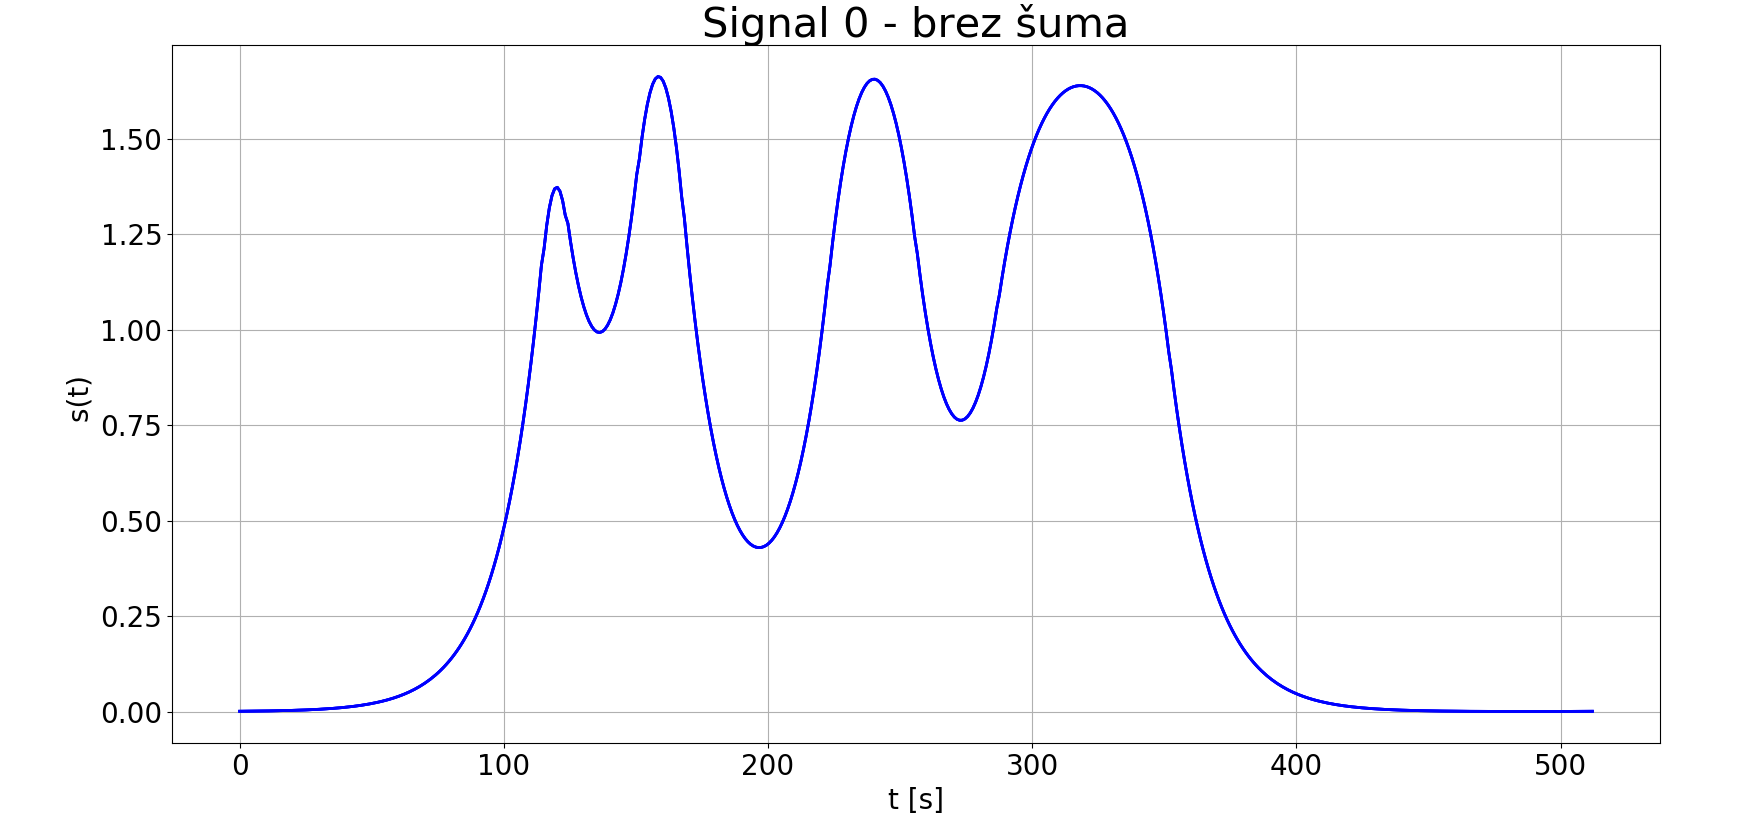
\includegraphics[width=8cm]{druga_prvi.png}
\includegraphics[width=8cm]{druga_prvi1.png}

\caption{Prikaz signalov}  
\end{figure}
\iffalse
\section{Statistika časov izumrtja}
\subsection{Poissonska porazdelitev umrlih}
Obravnamo eksponetni model, ki nam opisuje upad populacije $N$.
\begin{equation}
\frac{dN}{dt} = - \beta N
\end{equation}
Ker ne želimo zveznih rešitev, problem diskretizirajmo
\begin{equation}
\Delta N = - \beta  \Delta t N
\end{equation}
Sprememba populacijskega števila $\Delta N$, v nekam časovnem intervalu $\Delta t$ nam predstavlja povprečno število umrlih pri danem $N$. 
Pravo število umrlih pa je niz slučajnih procesov s verjetnostjo $p = -\beta N_0$ za smrt in $1 - p = 1 - (-\beta N_0)$ za preživetje, ki je porazdeljeno naključno po binomski porazdelitvi za neko časovni interval $\Delta t$, ki nam viša verjetnost smrti
\begin{equation}
P(x = \Delta N) = \binom{N_0}{\Delta N} (-\beta \Delta t )^{\Delta N } (1 - (- \beta \Delta t))^{N_0 - \Delta N}
\end{equation} 
povprečna vrednost umrlih je 
\begin{equation}
\lambda = N_0 p = -N_0 \beta \Delta t
\end{equation}
Če je število osbekov $N_0$ veliko in verjetnost $ -\beta \Delta t $ majhna se prevede binomska porazdelitev v \textbf{Poissonsko} porazdelitev
\begin{equation}
P(x) = \frac{\lambda^x e^{-\lambda}}{x!}
\end{equation}
pri čemer je x število dogodkov (število umrlih) in $\lambda = \beta \Delta t N$ povprečno število dogodkov na časovnem intervalu.
\subsection{Model I - Preprost model umirajoči model}
Naše populacijske modele lahko torej poissonsko izžrebamo, če poznamo njihove povprečne vrednosti, ki jih dobimo s diskretizacijo enačb.
\begin{figure}[H]
\centering

  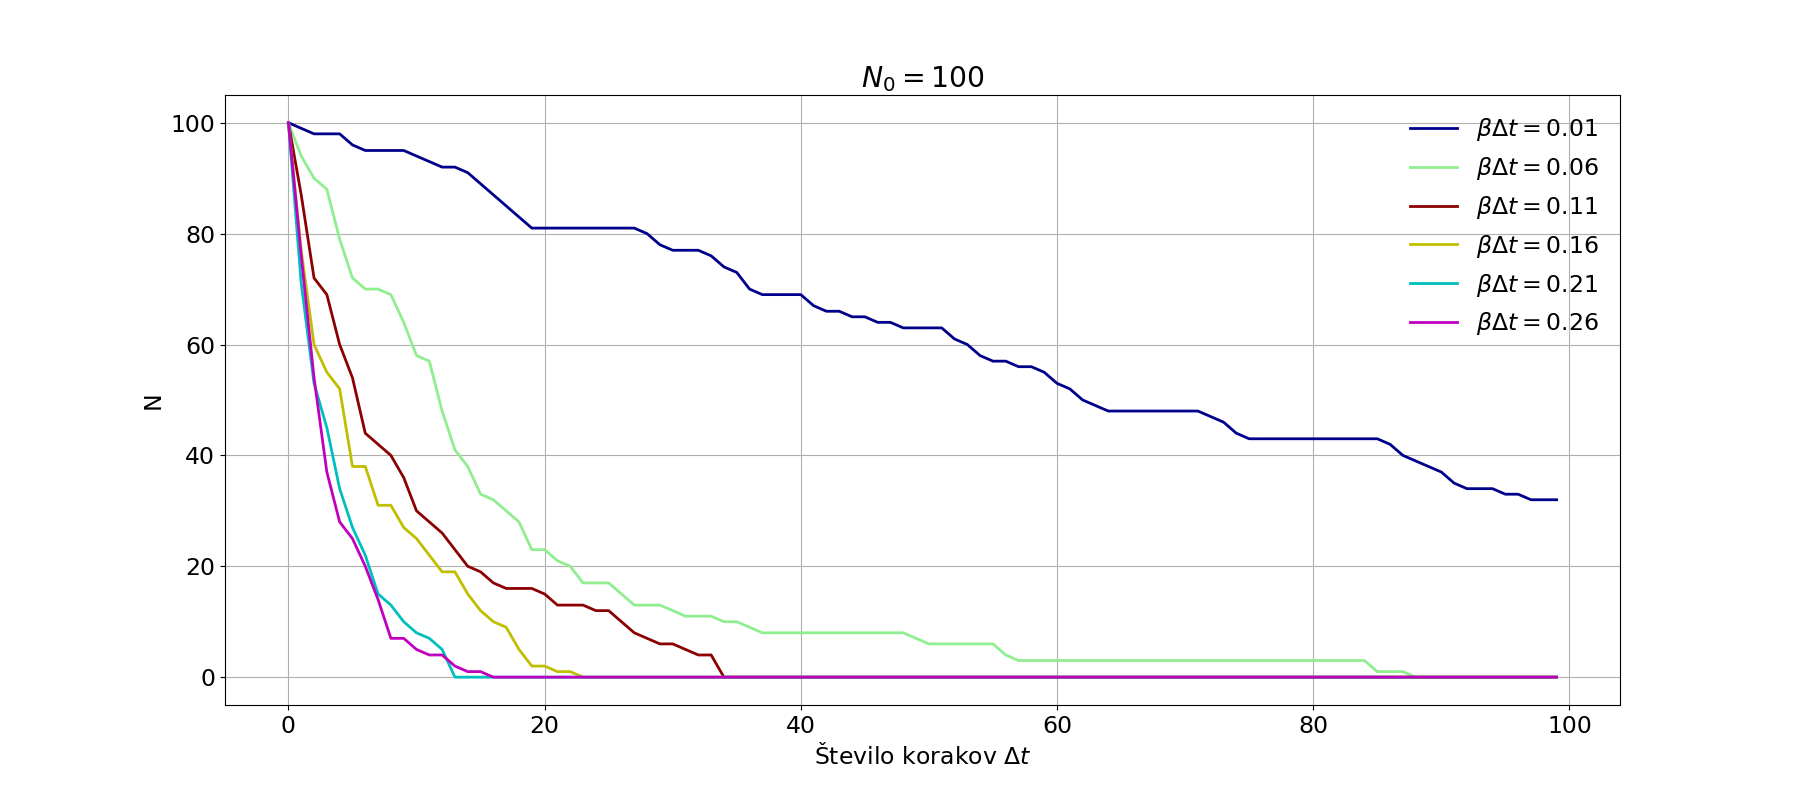
\includegraphics[width=18cm, height=4.5cm]{Umiranje_1.png}
   \caption{Umirajoč model, pri različnih vrednostih $\beta \Delta t$, že takoj vidimo, da je s višanjem parametra čas izumrtja vedno krajši.}
 \end{figure}
Vidimo, da zgornje rešitve niso zvezne, ker so $N$ le cela števila. Sedaj si poglejmo kaj se zgodi ko simulacijo pri fiksnem $\beta \Delta t$ poženemo večkrat.
\begin{figure}[H]
\centering

  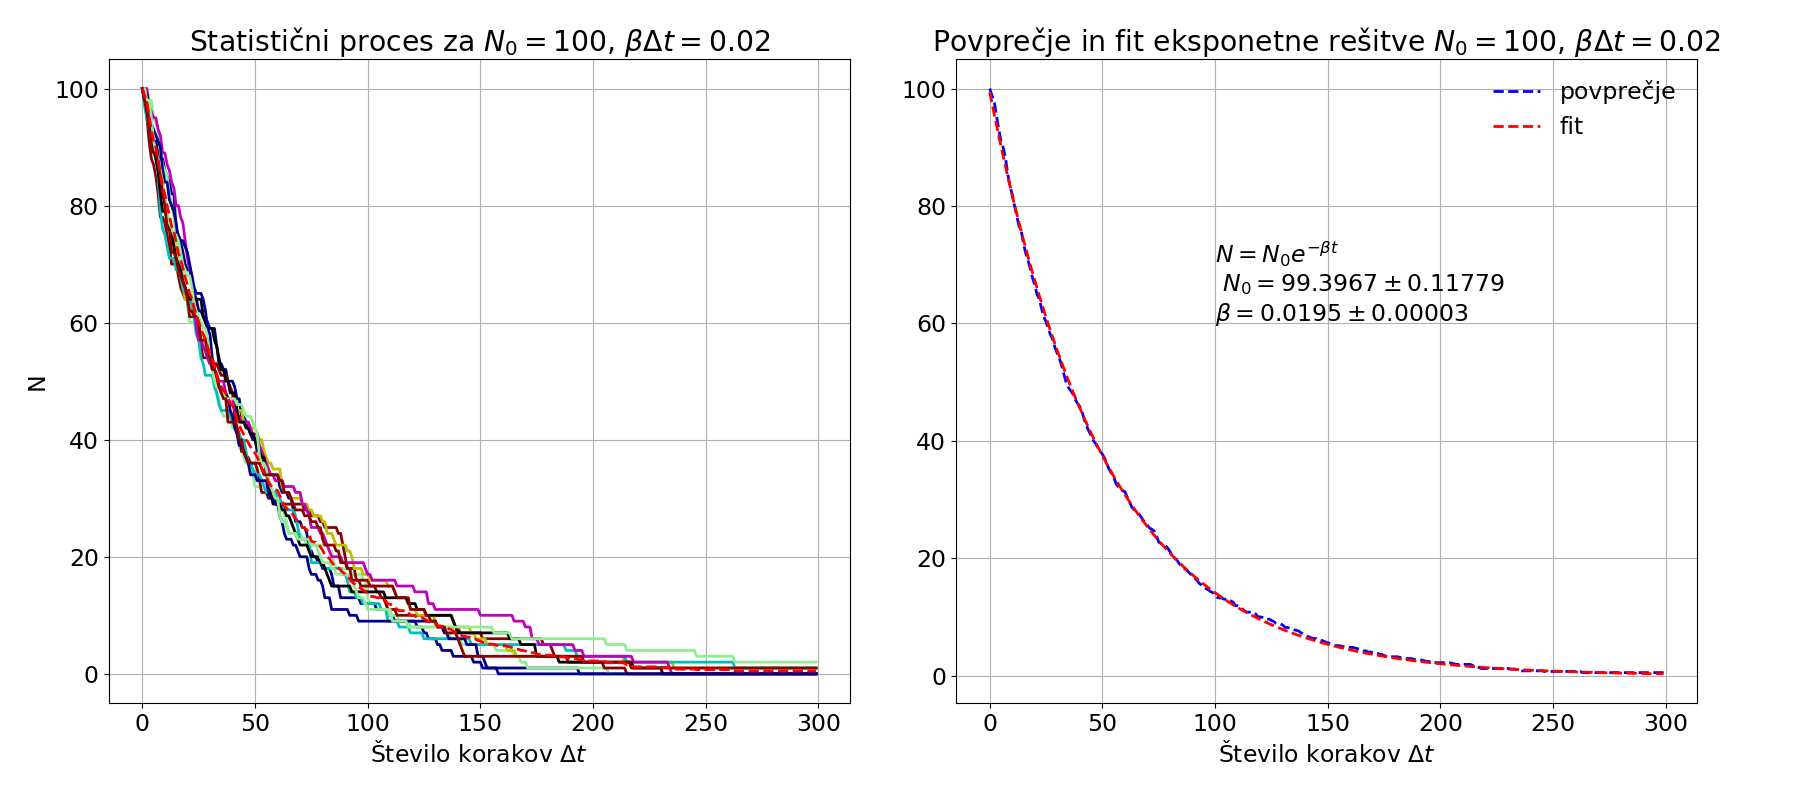
\includegraphics[width=18cm, height=6cm]{Umiranje_1_statisticni_proces.png}
   \caption{Levo, vidimo da je zaradi žrebanja proces izumrtja vsakič malo drugačne. Desno je izpovprečen graf in fit eksponentne krivulje nanj. \textbf{Vidimo, da s poissonskim procesom res lahko opišemo populacijske modele, saj izluščeni parametri usterzajo predpostavljenimi.}}
  
 \end{figure}
 \subsection{Velikost populacije}
 Zanima nas kako začetna velikost populacije vpliva na potek populacijske sheme.
 
 \begin{figure}[H]
\centering

  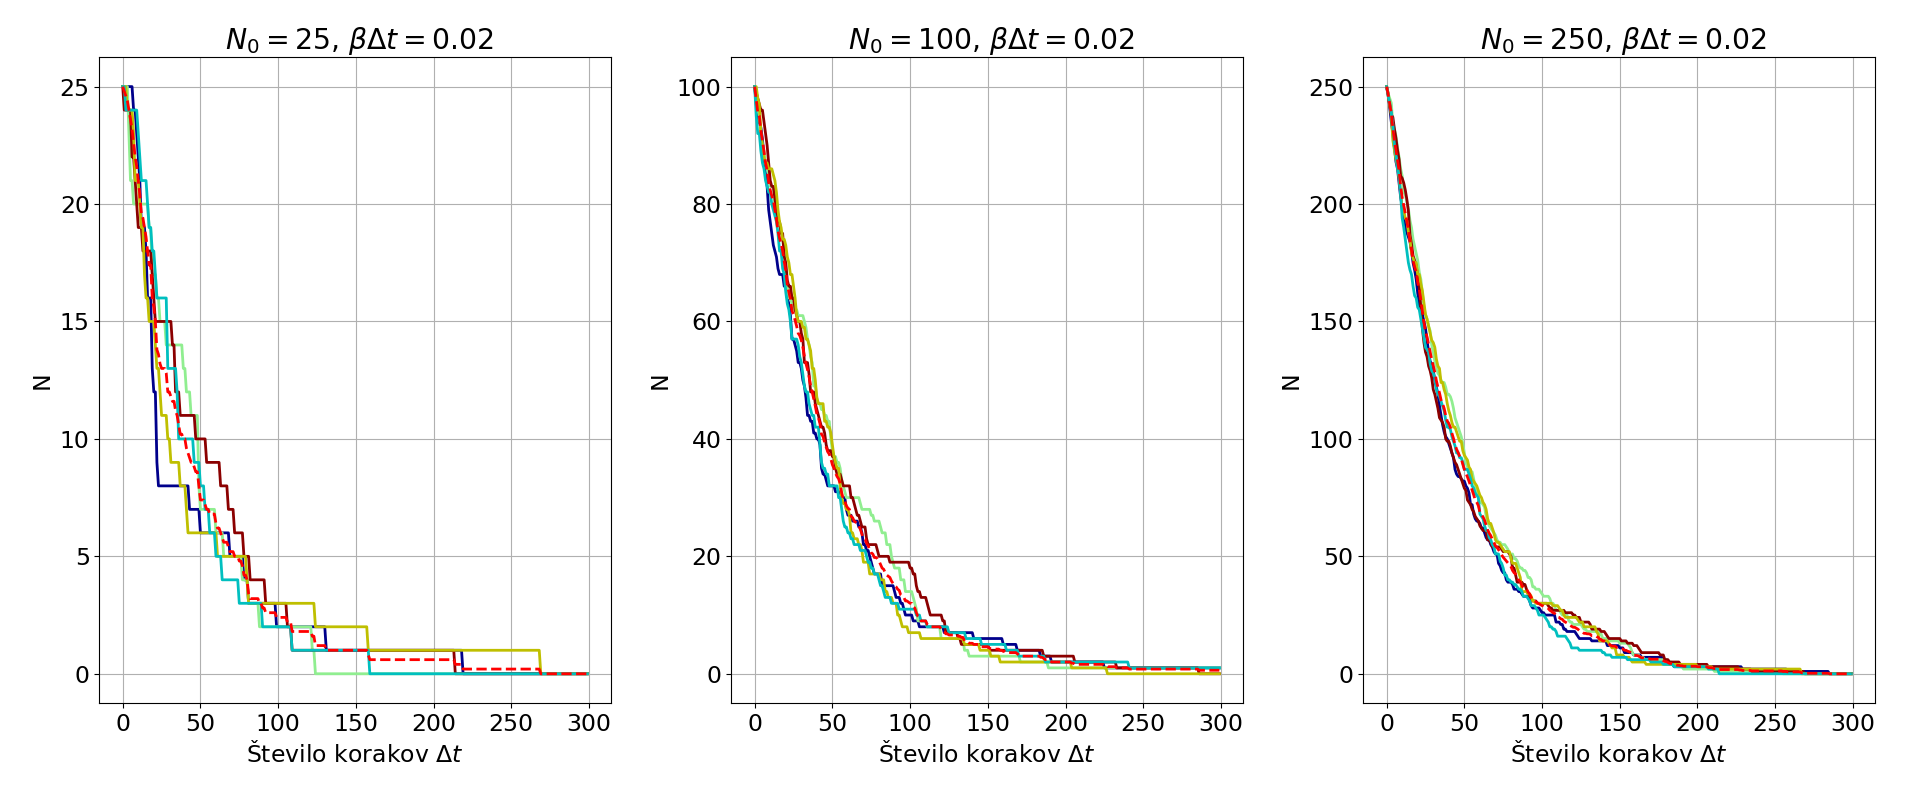
\includegraphics[width=18cm, height=6cm]{Umiranje_1b.png}
   \caption{Z večanjem populacije so skoki med časovnimi intervali vse bolj zvezni.}
  
 \end{figure}

 \subsection{Model II - Združeni modeli}
Sedaj pa si poglejmo še rojstvo in smrt
\begin{equation}
\frac{dN}{dt} = + \beta_r N - \beta_s N
\end{equation}
Vemo da lahko zgronjo enačbo prepišemo v 
\begin{equation}
\frac{dN}{dt} = - \beta_{eff} N
\end{equation}
,kjer je $\beta_{eff} = \beta_r - \beta_s$ in tako dobimo efektivno upadanje oziroma naraščanje populacije. Tak proces pa simuliramo tako, da izžrebamo dva poissonska procesa, 
\begin{equation}
P (x) =  P( x, \lambda = + \beta_r N \Delta t) + P (x , \lambda = - \beta_s N \Delta t)
\end{equation}


 \begin{figure}[H]
\centering

  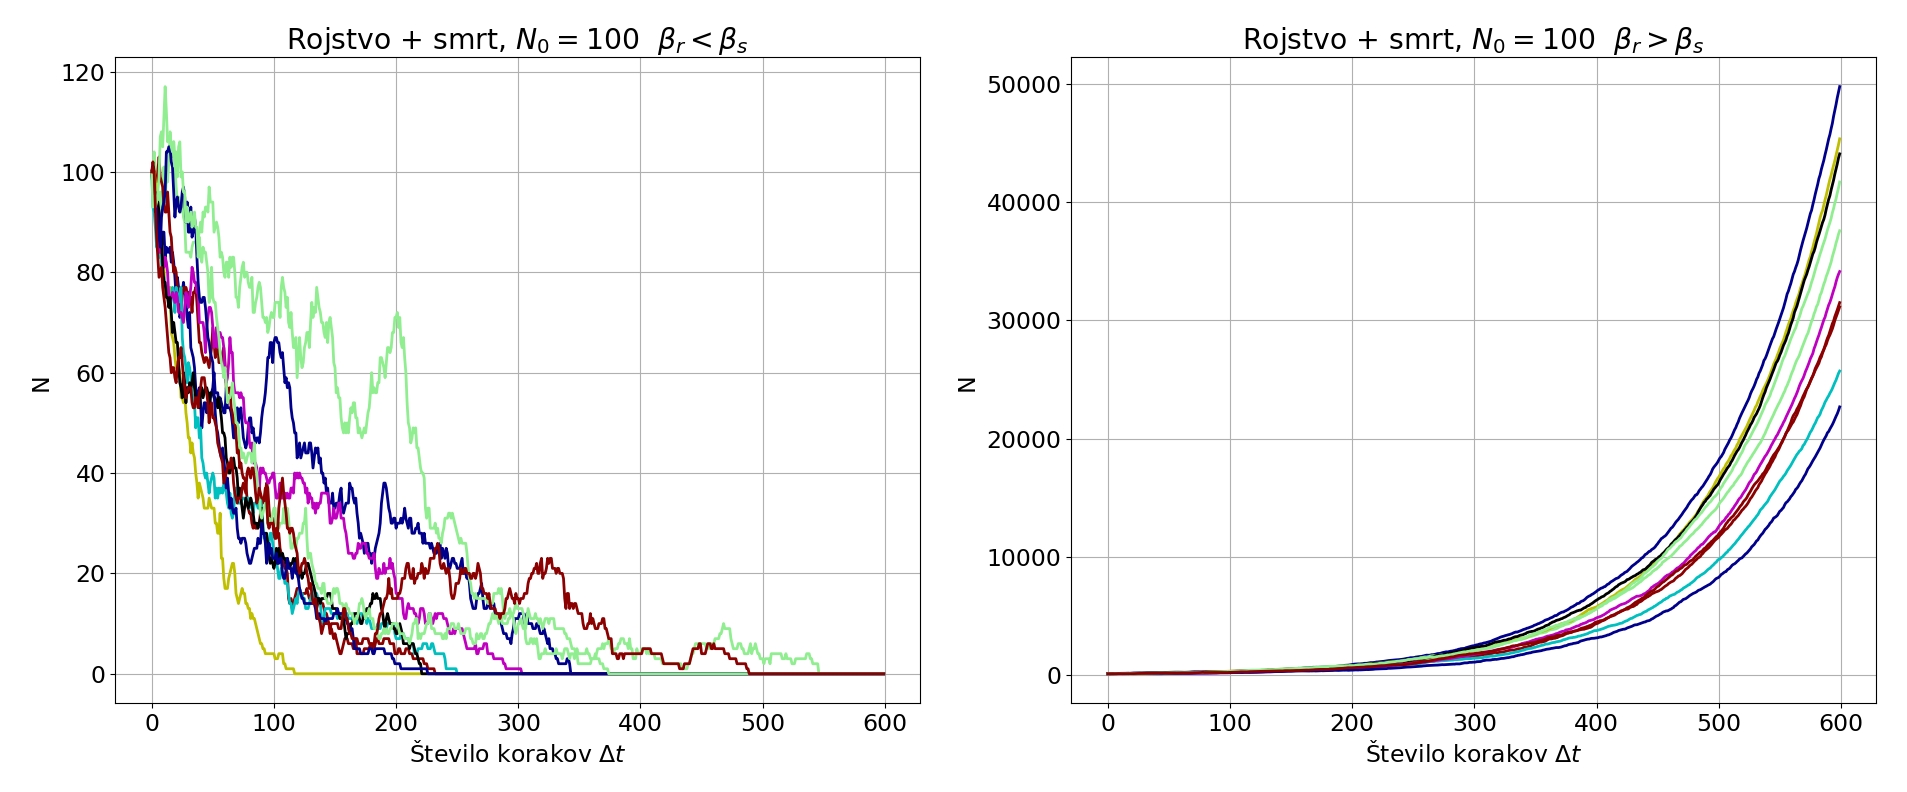
\includegraphics[width=18cm, height=6cm]{Rojevanja_2.png}

   
 \end{figure}
  \begin{figure}[H]
\centering

  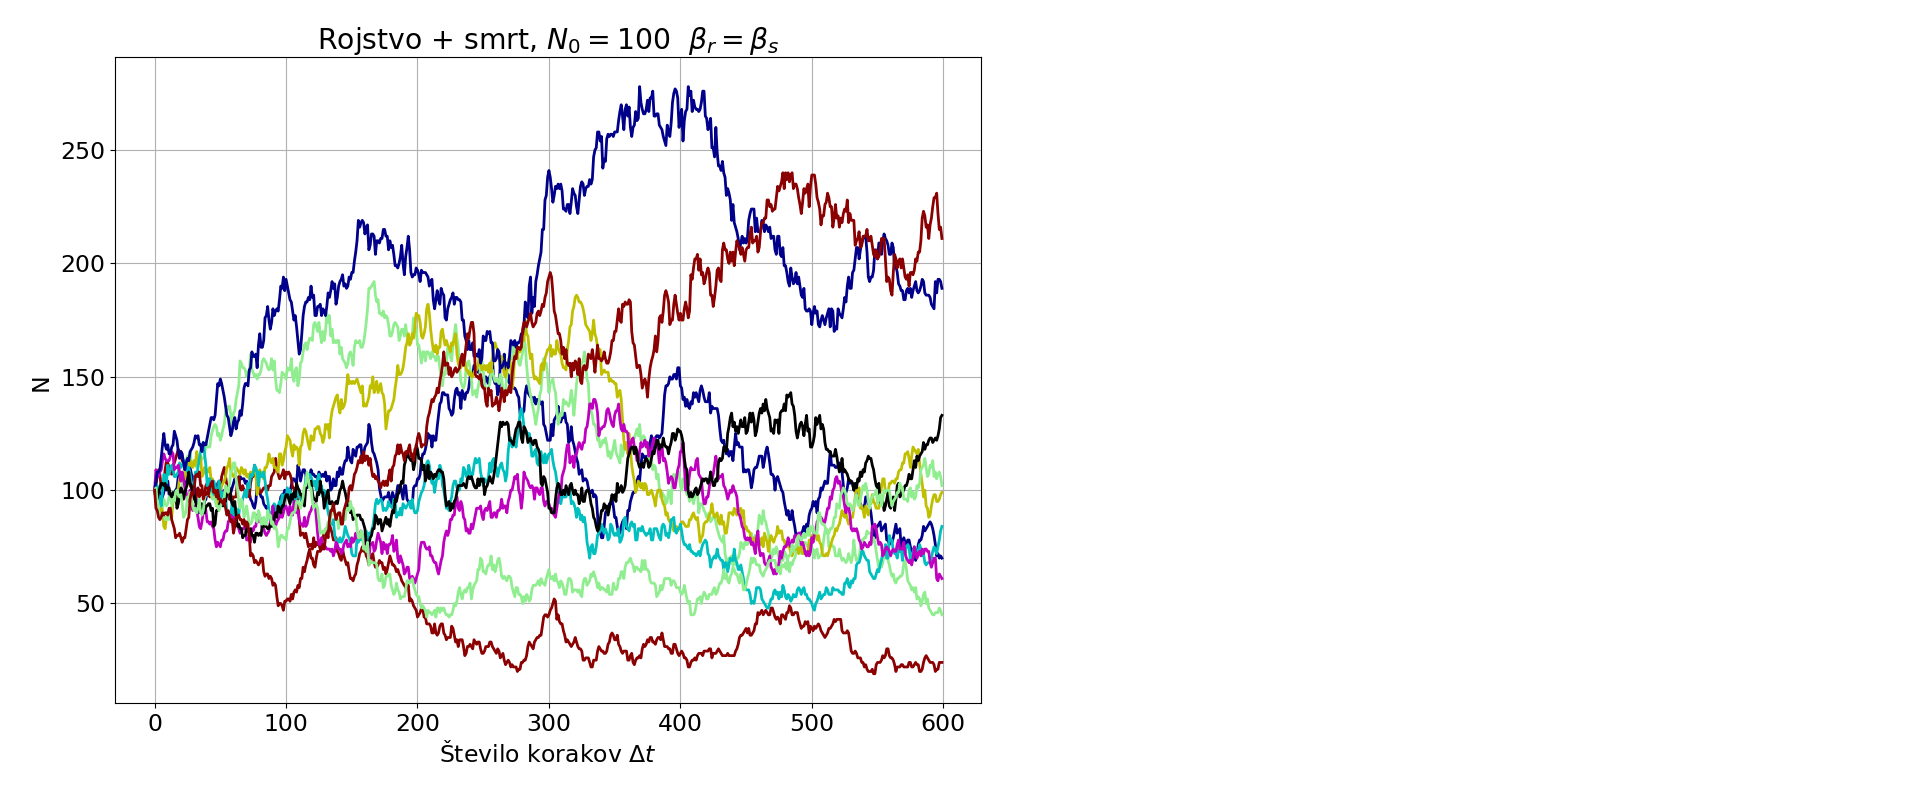
\includegraphics[width=18cm, height=6cm]{Rojevanja_1b.png}
     \caption{Pri modelu rojevanja in umiranja je populacijska shema odvisna od konstant $\beta_r$ in $\beta_s$. Če sta enaki potem dobimo v povprečju }
 \end{figure}

\subsection{Statistika časov izumrtja}
Populacija počasi izumira, zato nas zanima kako so porazdeljeni časi izumtrja. Ker je čas izumtrja konvolucija več poissonskih procesov, pričakujemo da bodo po centralnem limitnem teoremu porazdeljeni gausovo.
 \begin{figure}[H]
\centering

  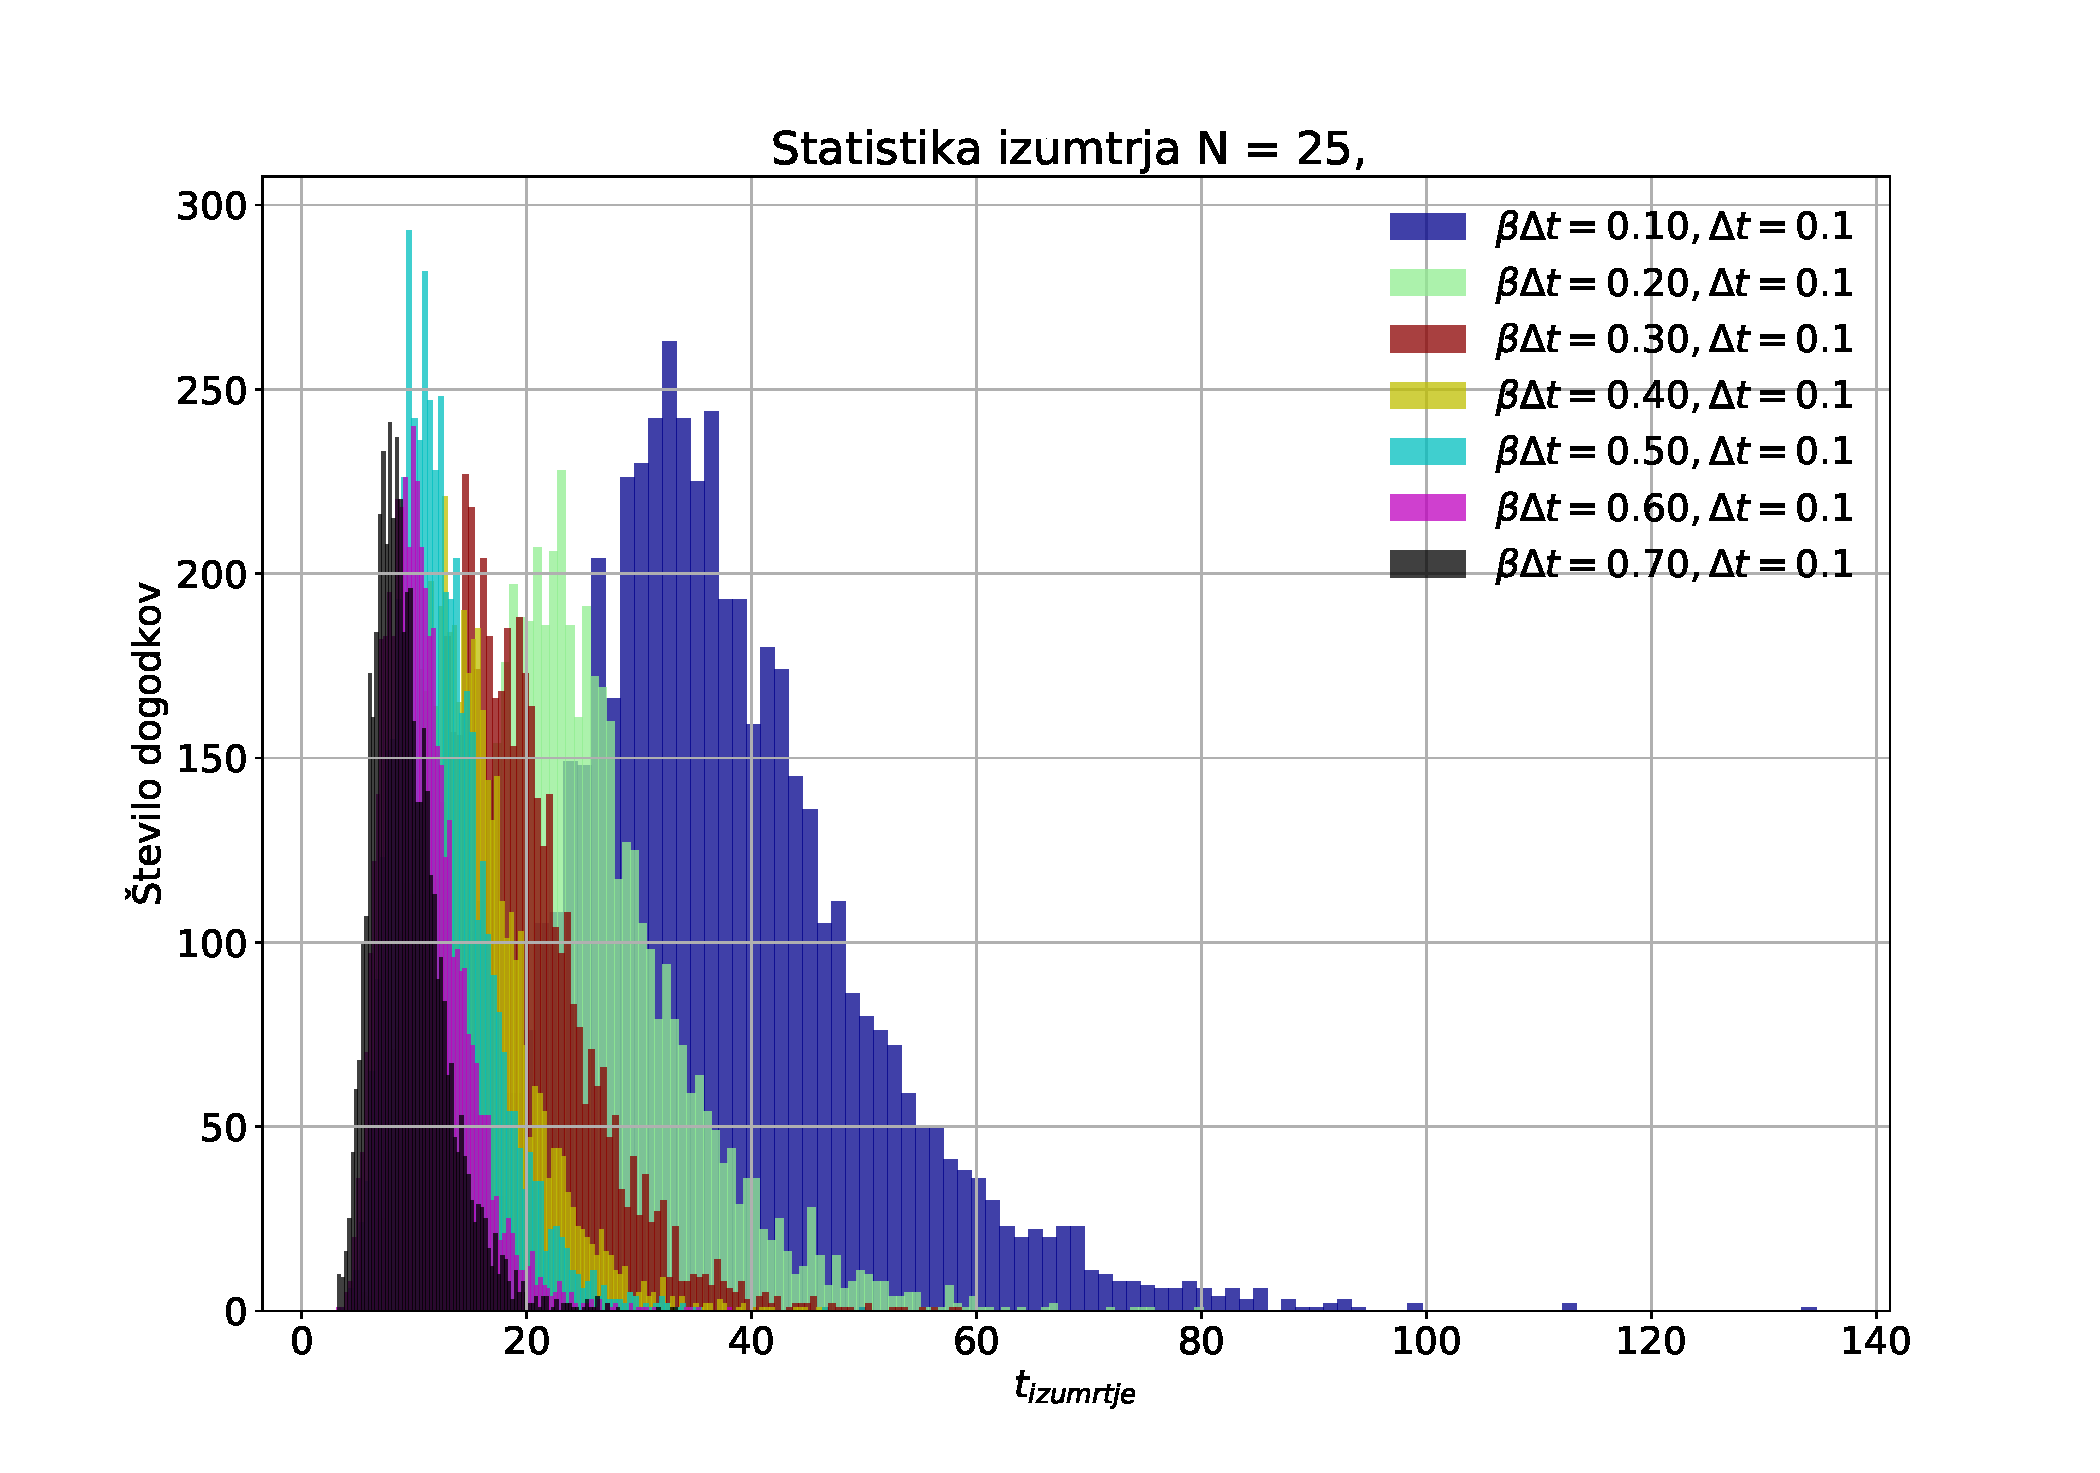
\includegraphics[width=16cm, height=5cm]{prva_drugidel1b.pdf}
    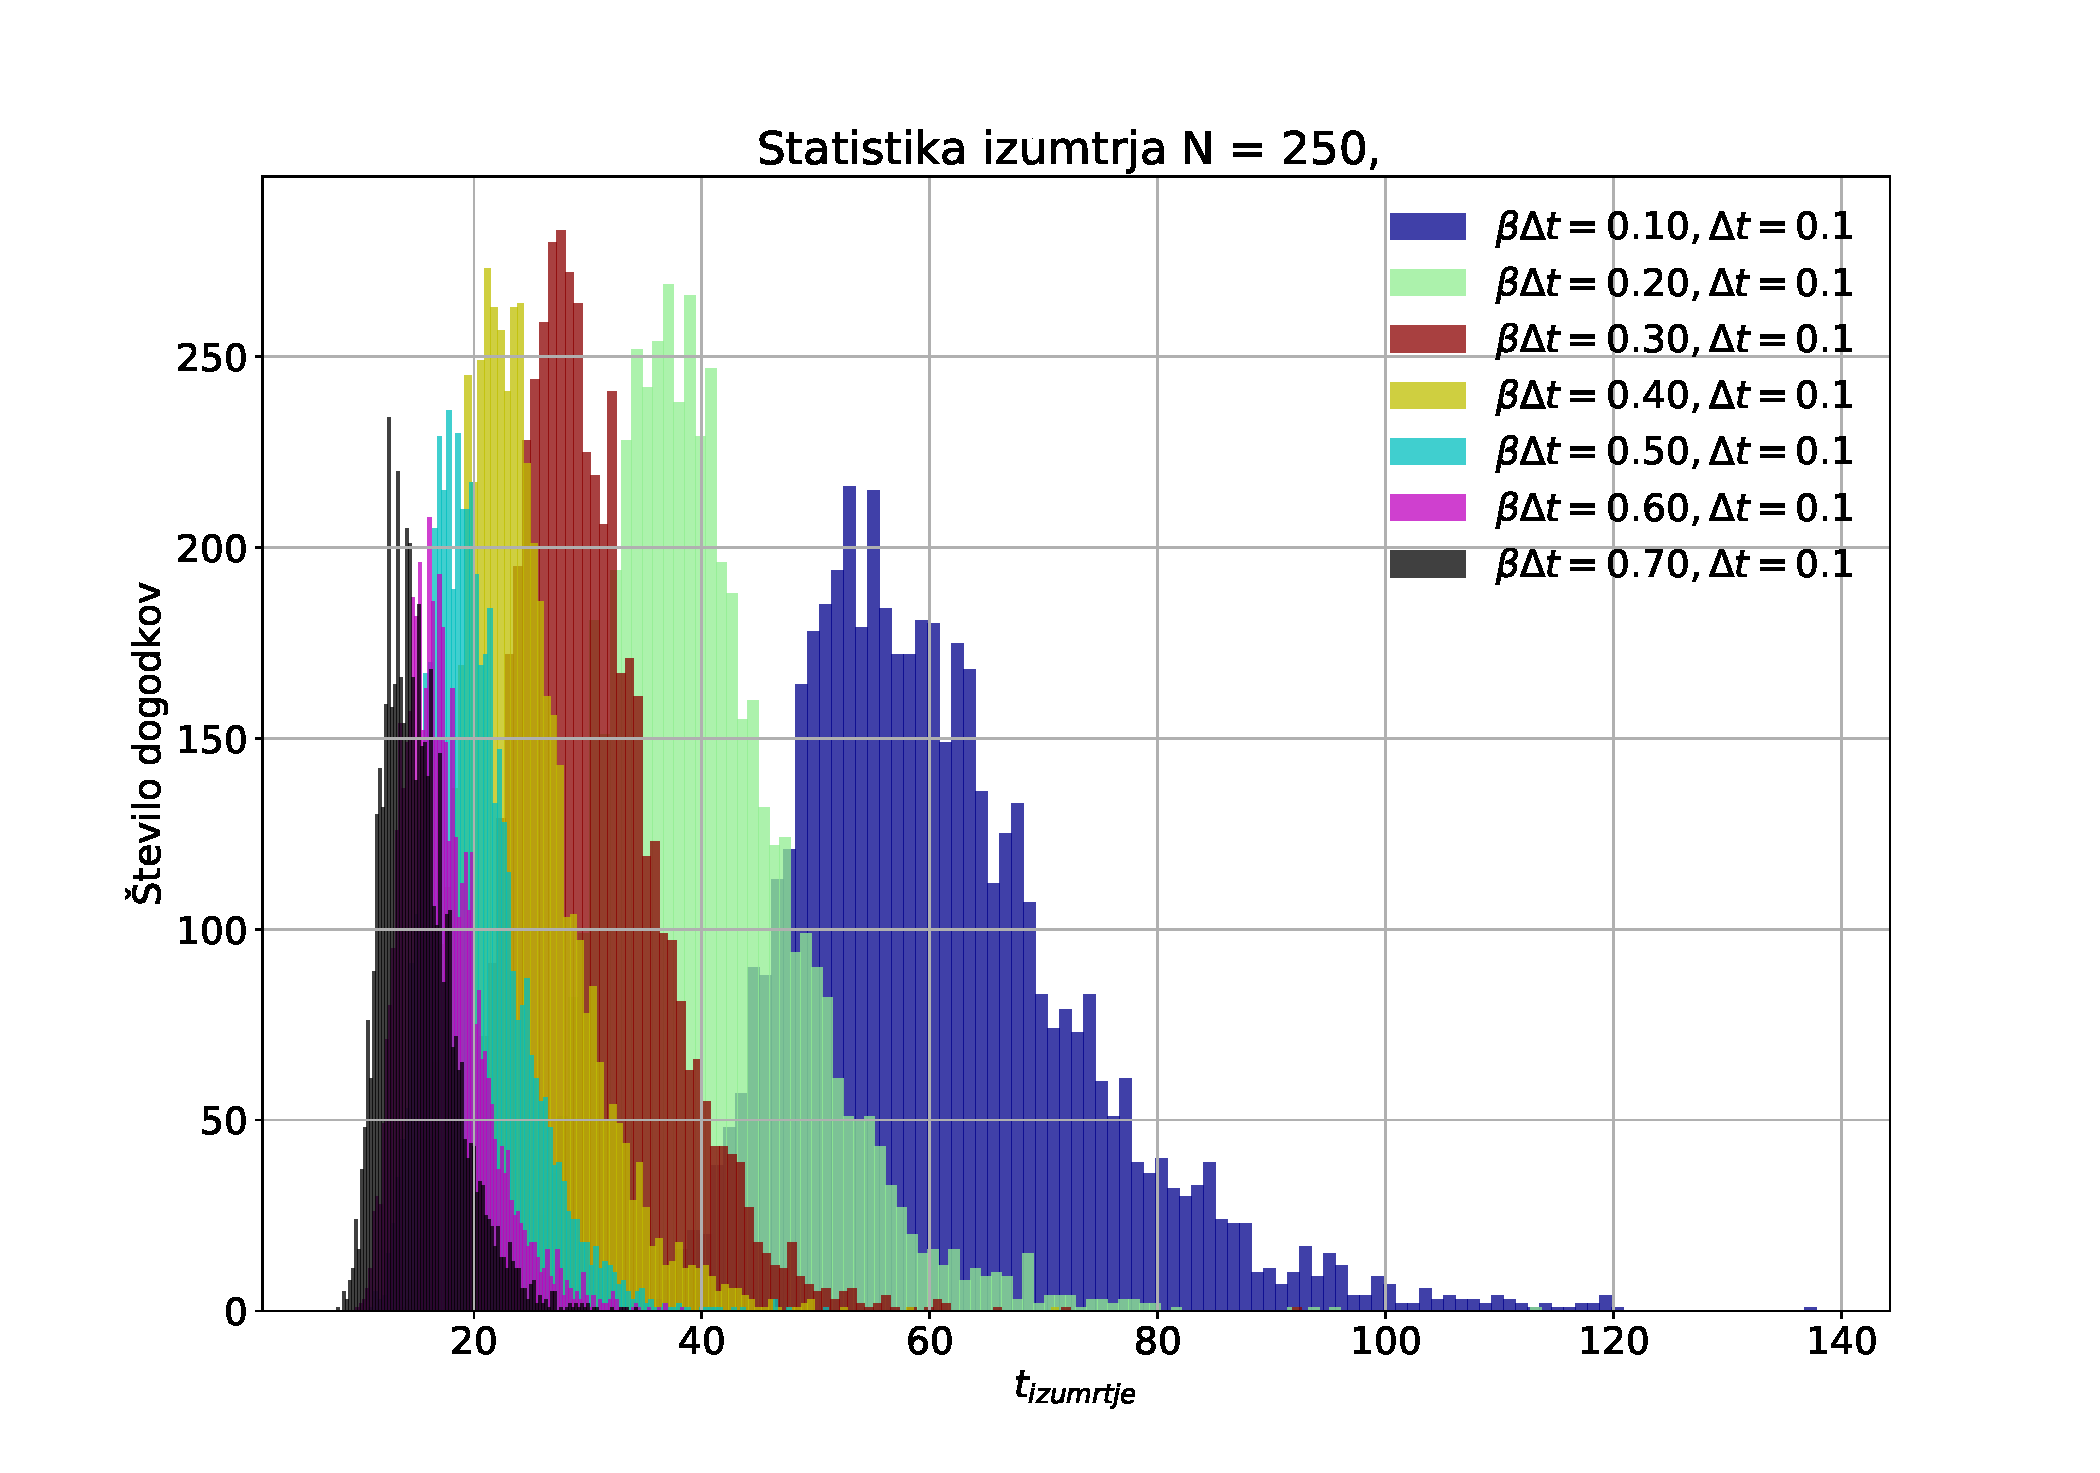
\includegraphics[width=16cm, height=5cm]{prva_drugidel1c.pdf}
   \caption{Model 1. Za začetno populacijo $N = 250$ in $N = 25$ simuliramo umiranje $n=5000$ krat in narišemo histogram. Vidimo, da je čas izumrtja res porazdeljena normalno in tako lahko odčitamo povprečni čas izumrtja populacije. Hkrati vidimo, da so za večjo populacijo časi povprečni časi daljši, kar bomo tudi preverili v nadaljevanju.}
   
 \end{figure}
 
  \begin{figure}[H]
\centering
  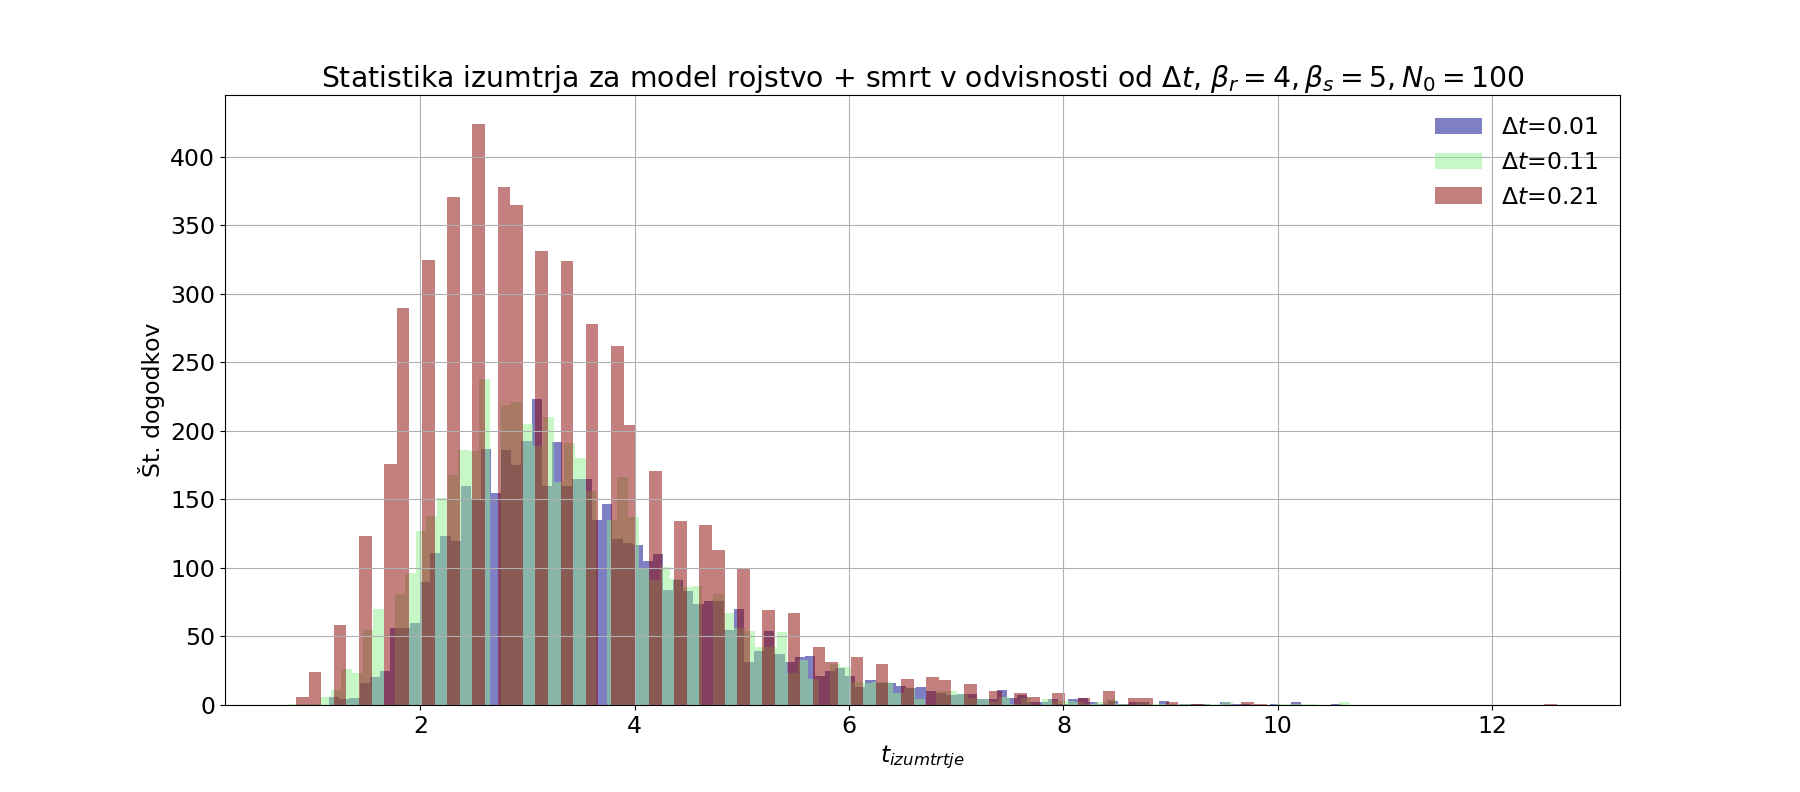
\includegraphics[width=16cm, height=5.5cm]{prva_tretji_del.png}
   \caption{Model 2. Statistika izumrtja v odvisnosti od časovnega razmaka. Vidimo da pri tem modelu časovni korak ne vpliva na čas izumtrja, časi pa se zanimivo pri višjih časovnih razmakih bolj zgostijo kar se odraža na rdečem histogramu, saj je razredov preveč. }   
 \end{figure}
 \subsection{Povprečni čas izmutrja}
Prikažimo sedaj izpovprečene čase izumtrja za različne vrednosti konstant $\beta$ in $\Delta t $, ter različno začetno populacijo.
   \begin{figure}[H]
\centering
  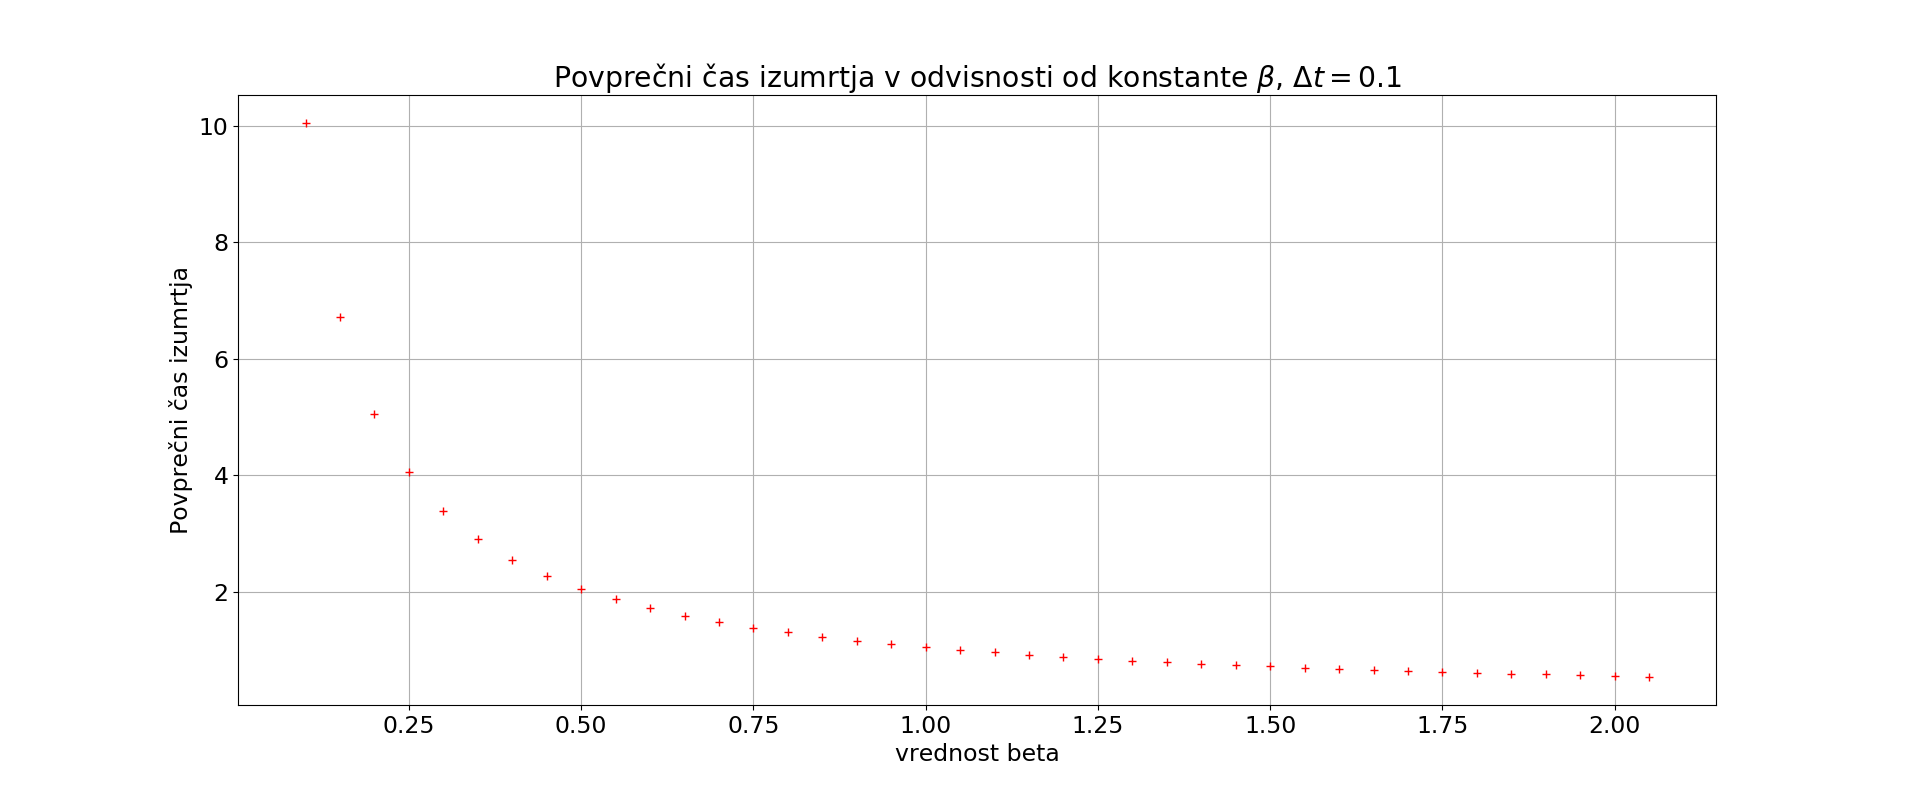
\includegraphics[width=16cm, height=4.5cm]{prva_povprecnicas.png}
   \caption{Model 1. Vidimo da je odvisnost časa izmutrja od $\beta$ eksponetna.}   
 \end{figure}
Poglejmo si še odvisnost povprečnega časa izumtrja od časovnega koraka $\Delta t$.
  \begin{figure}[H]
\centering
  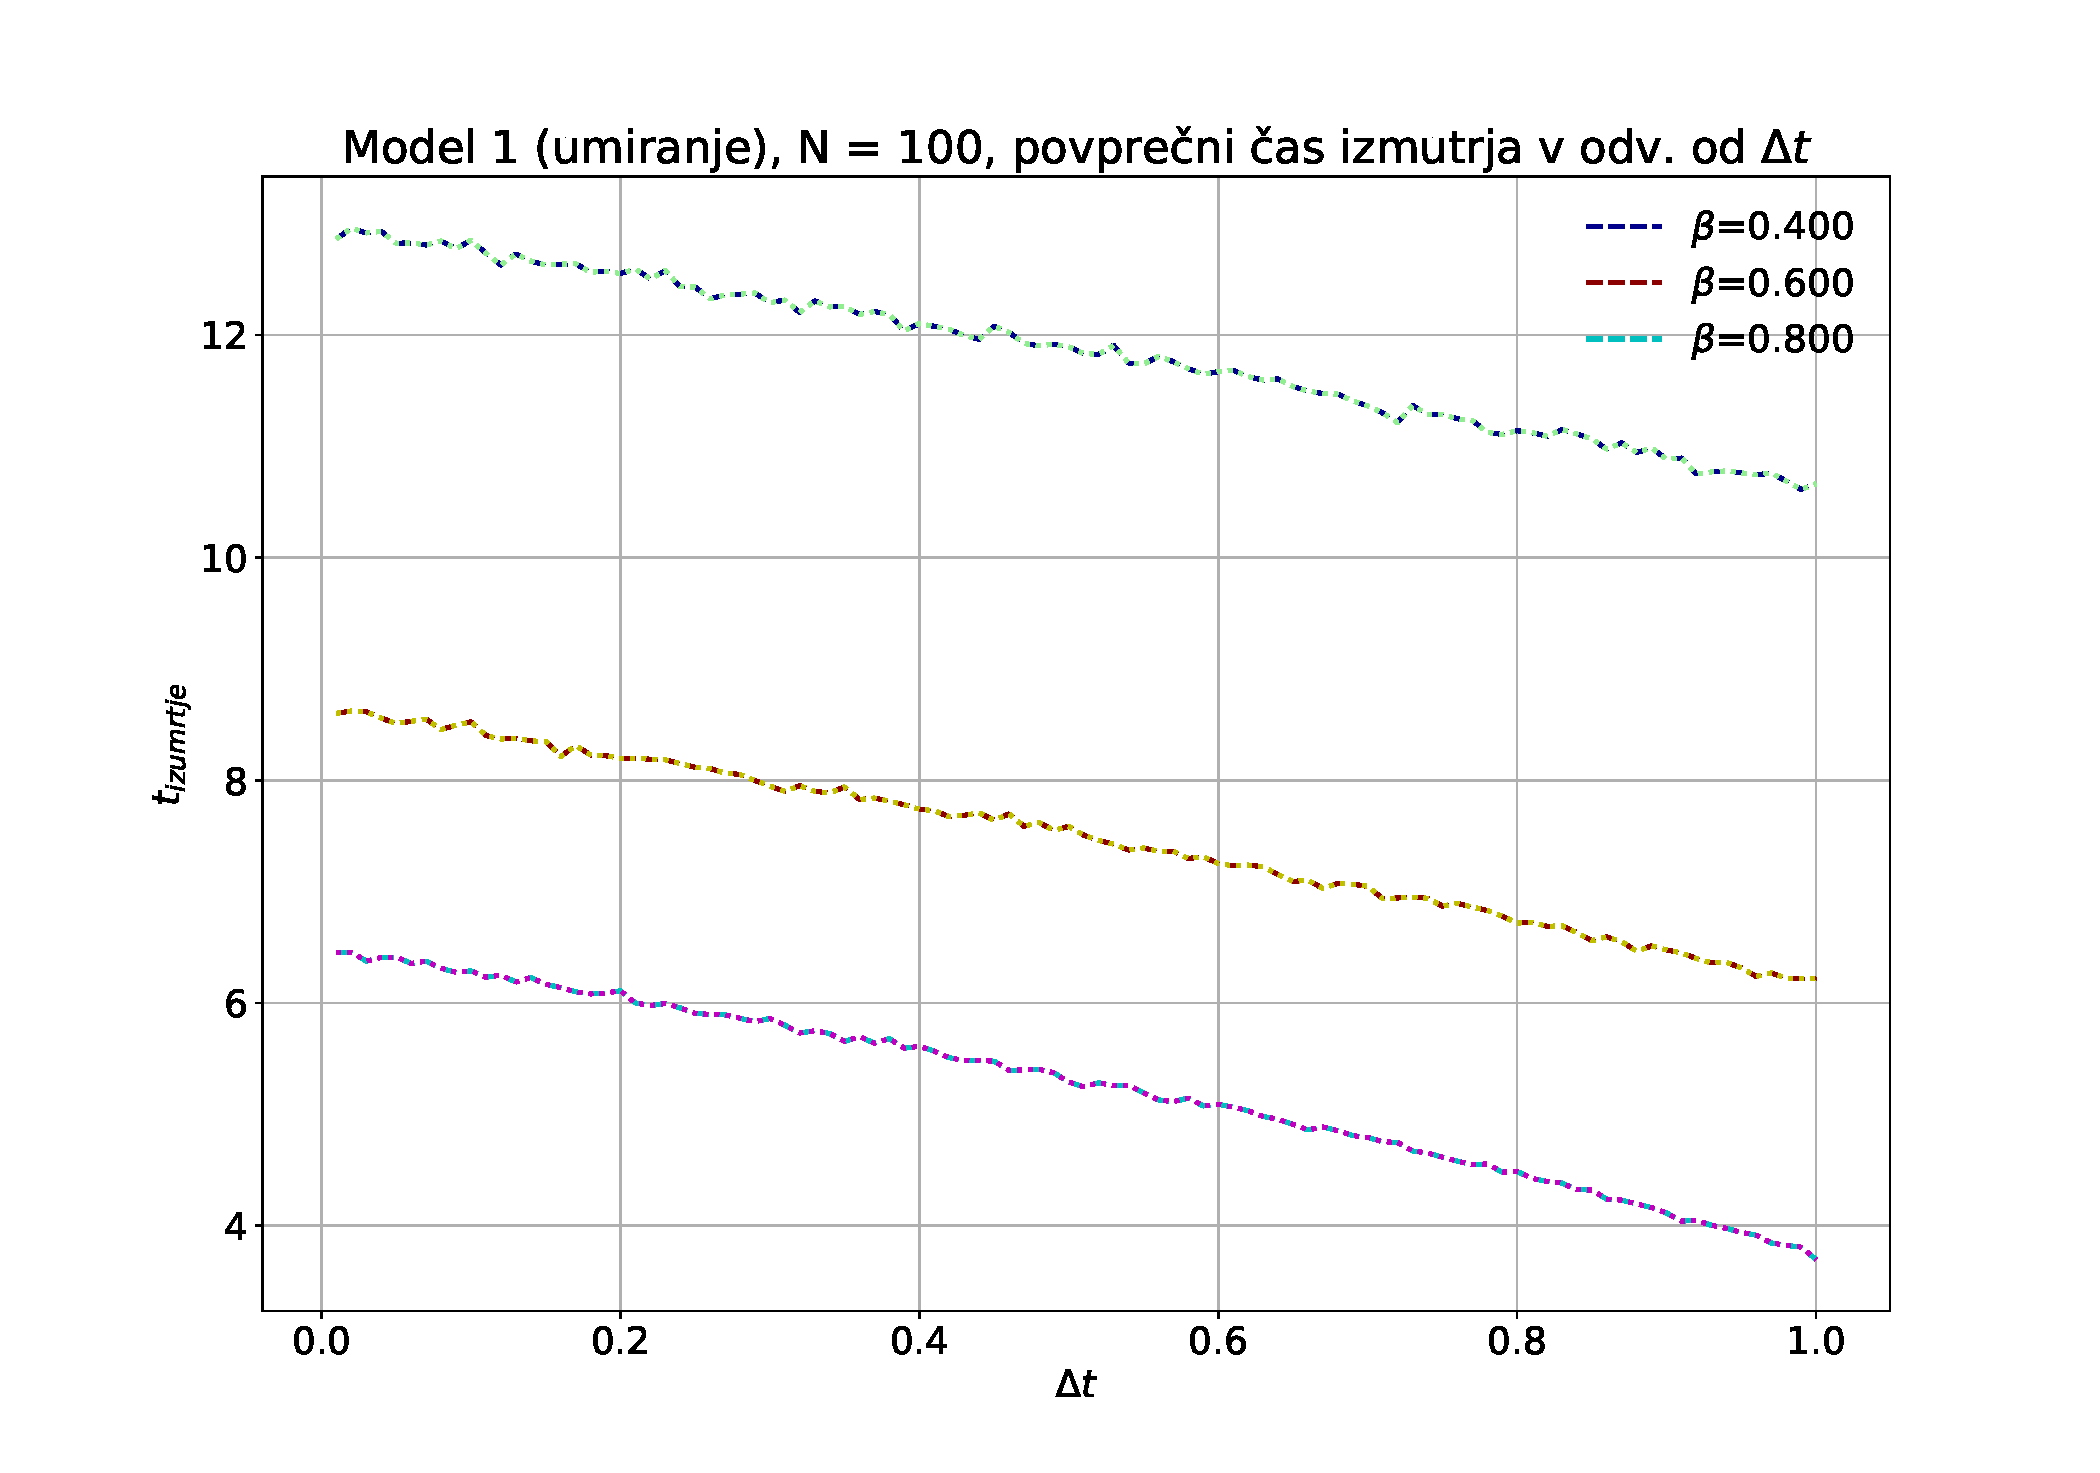
\includegraphics[width=8cm, height=6cm]{prva_tretji_del2.pdf}
    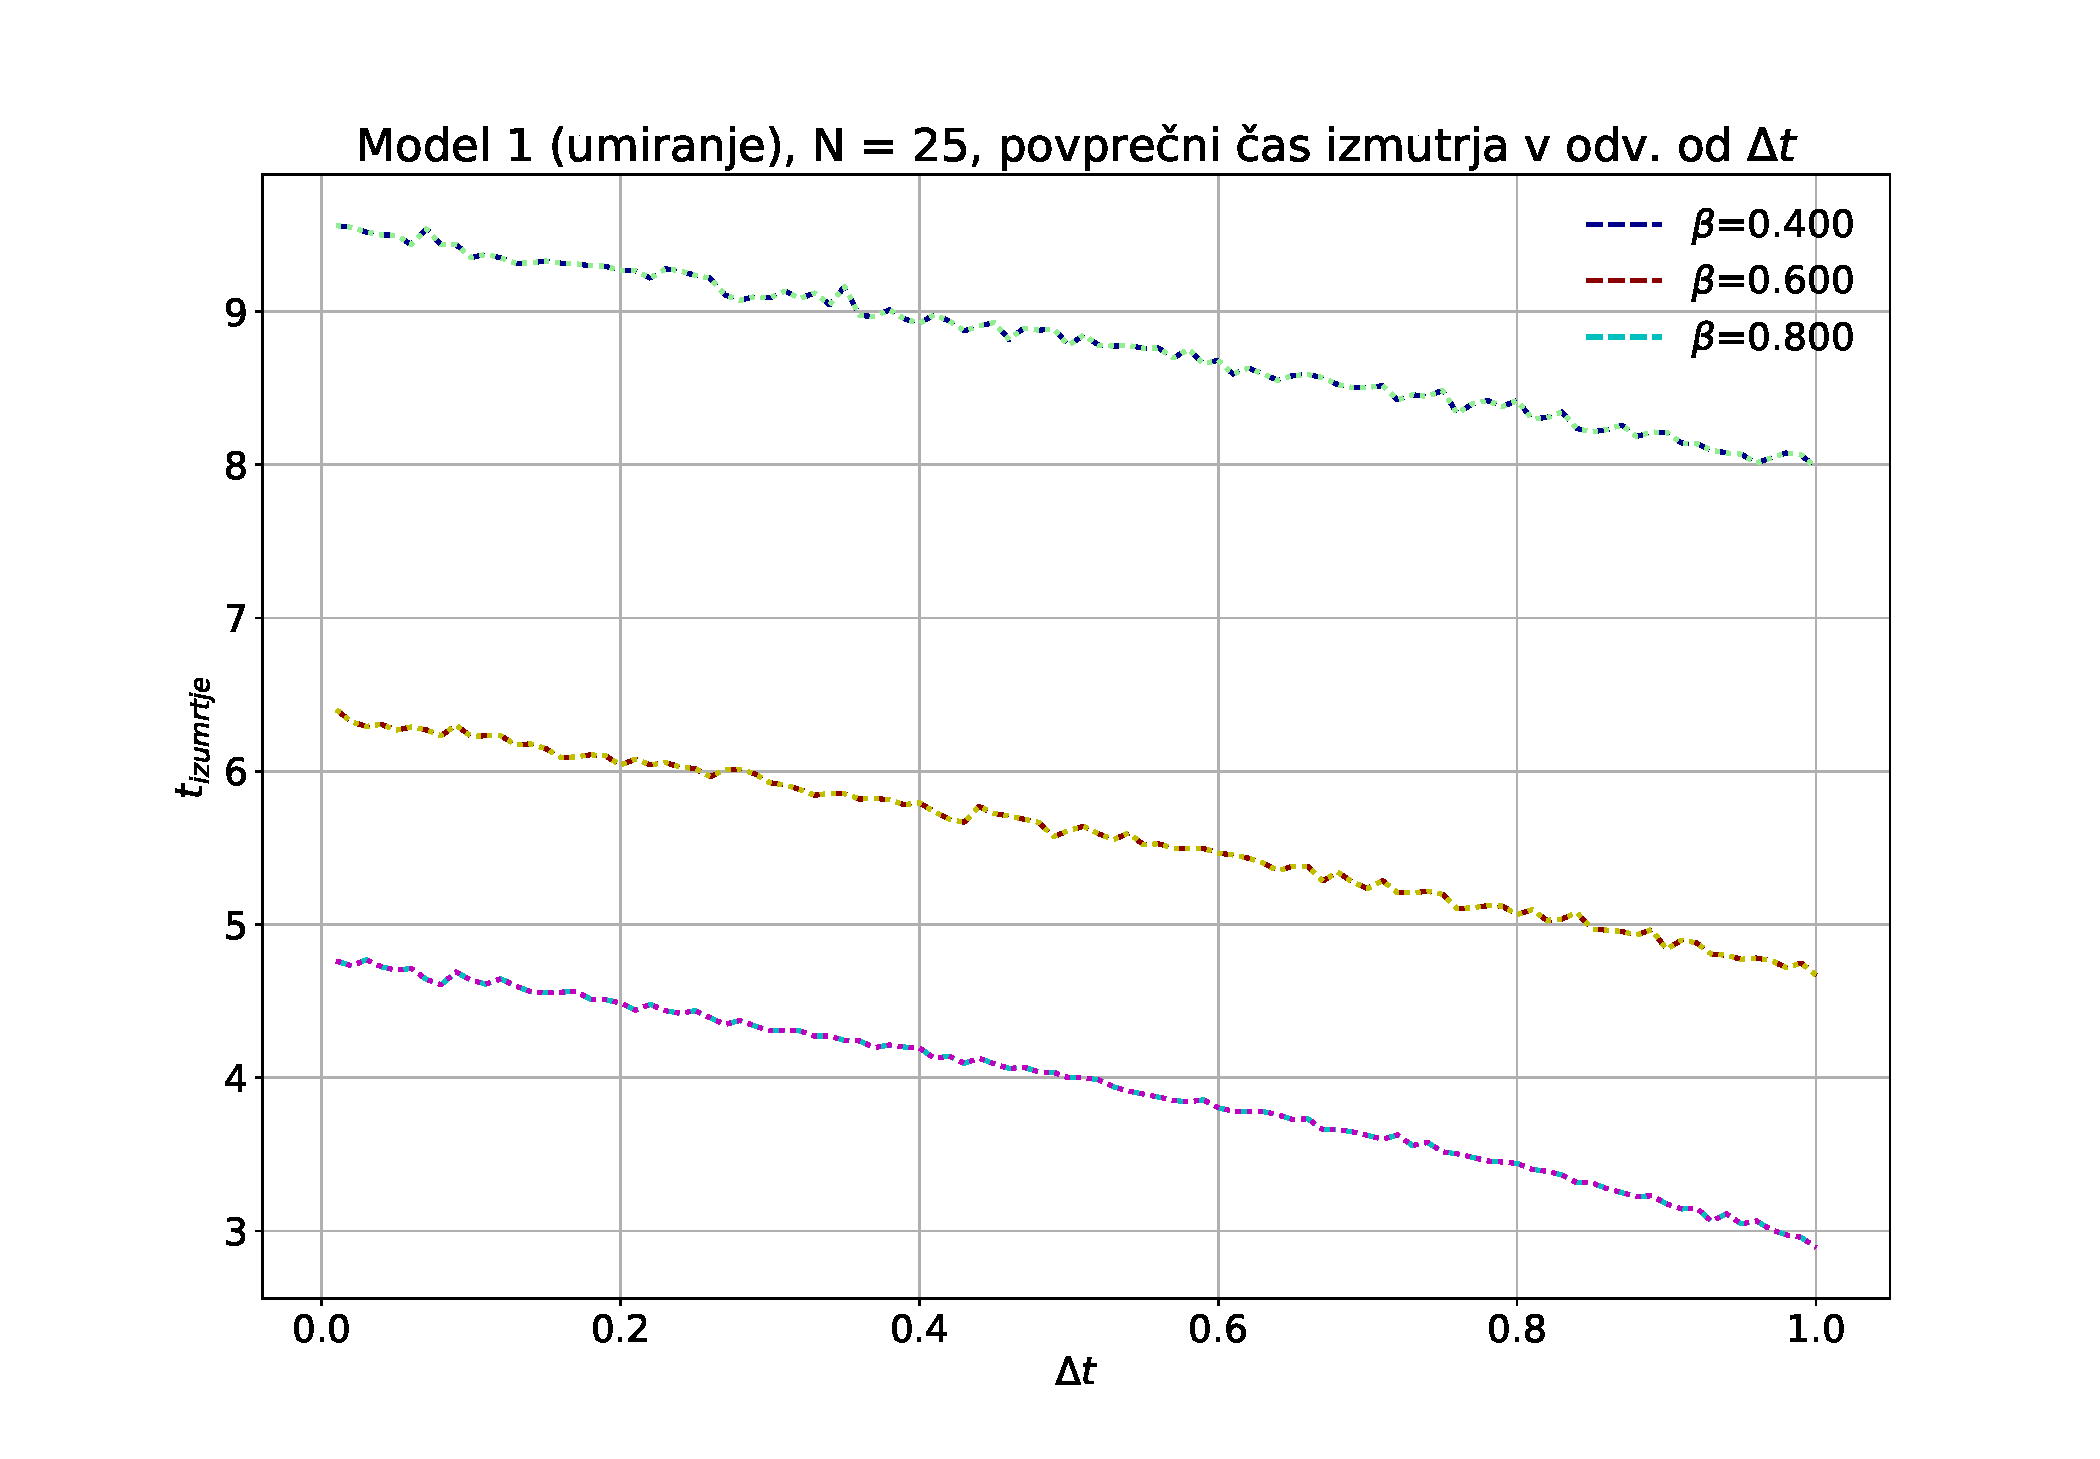
\includegraphics[width=8cm, height=6cm]{prva_tretji_del2b.pdf}
   \caption{Model I. Povprečni čas izumtrja v odvisnosti od razmika $\Delta t$ pričakovano pada, saj je če počakamo dlje časa več umrlih. Prav tako pada s naraščanjem bete.}   
 \end{figure}
  
   \begin{figure}[H]
\centering

  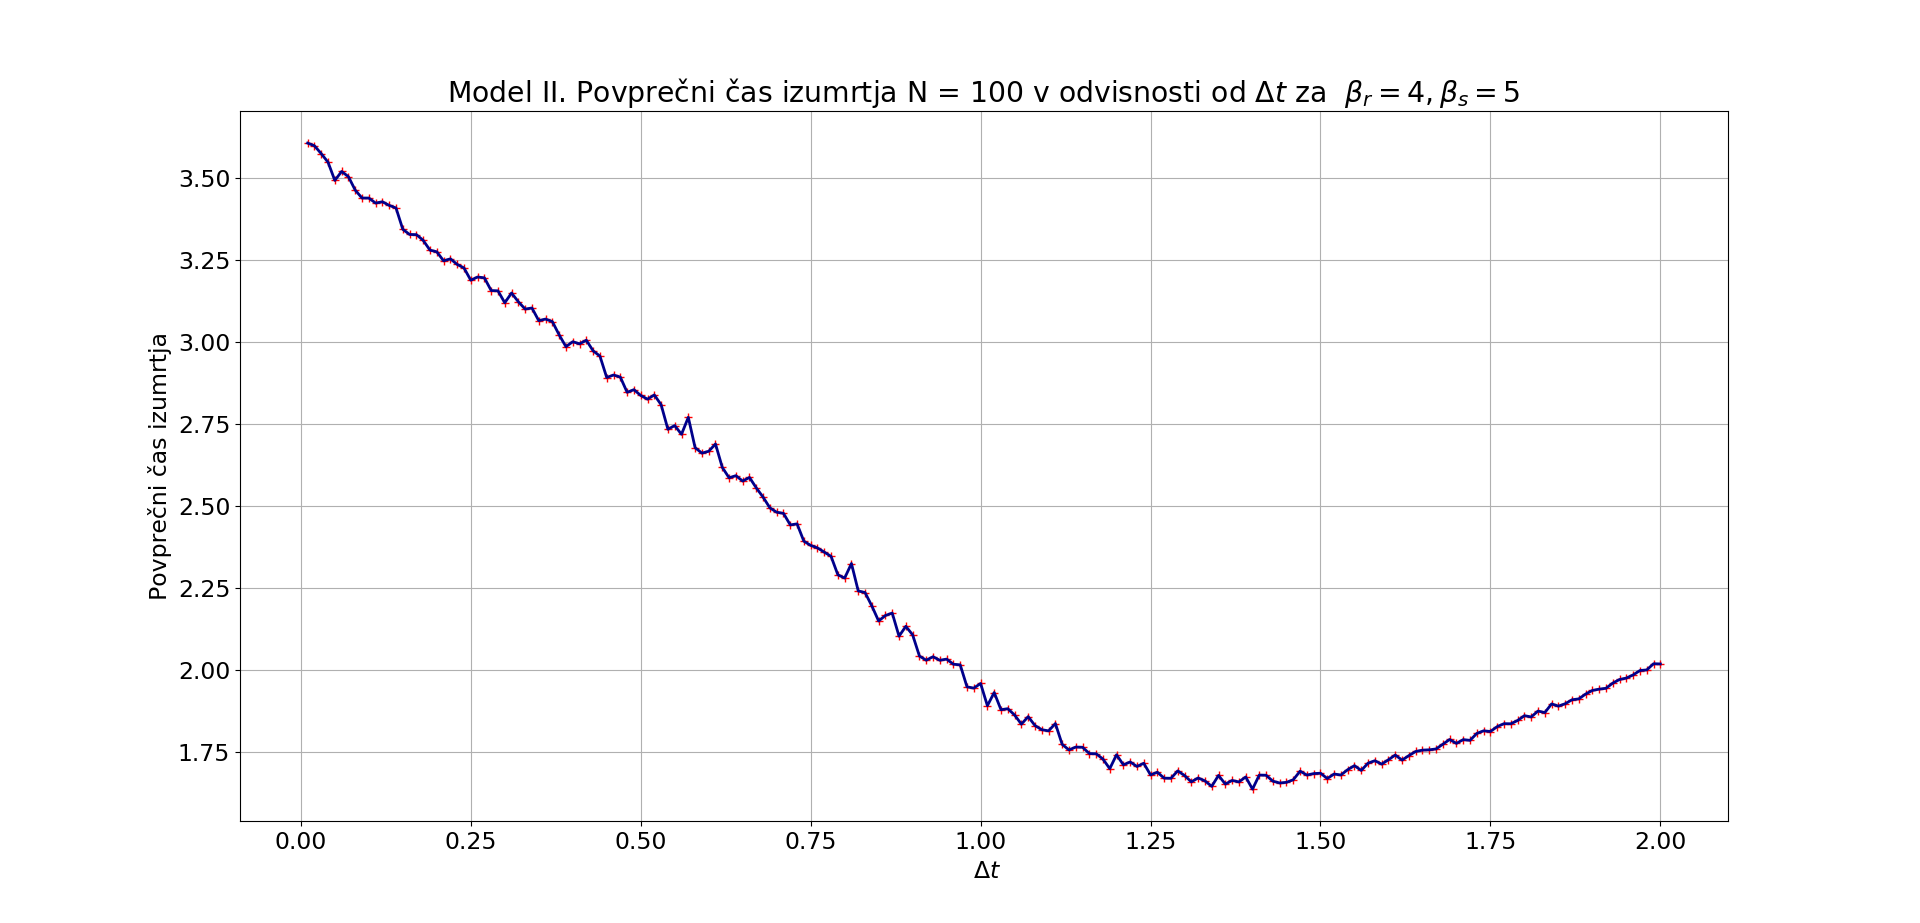
\includegraphics[width=18cm, height=5cm]{prva_tretji_del3.png}
  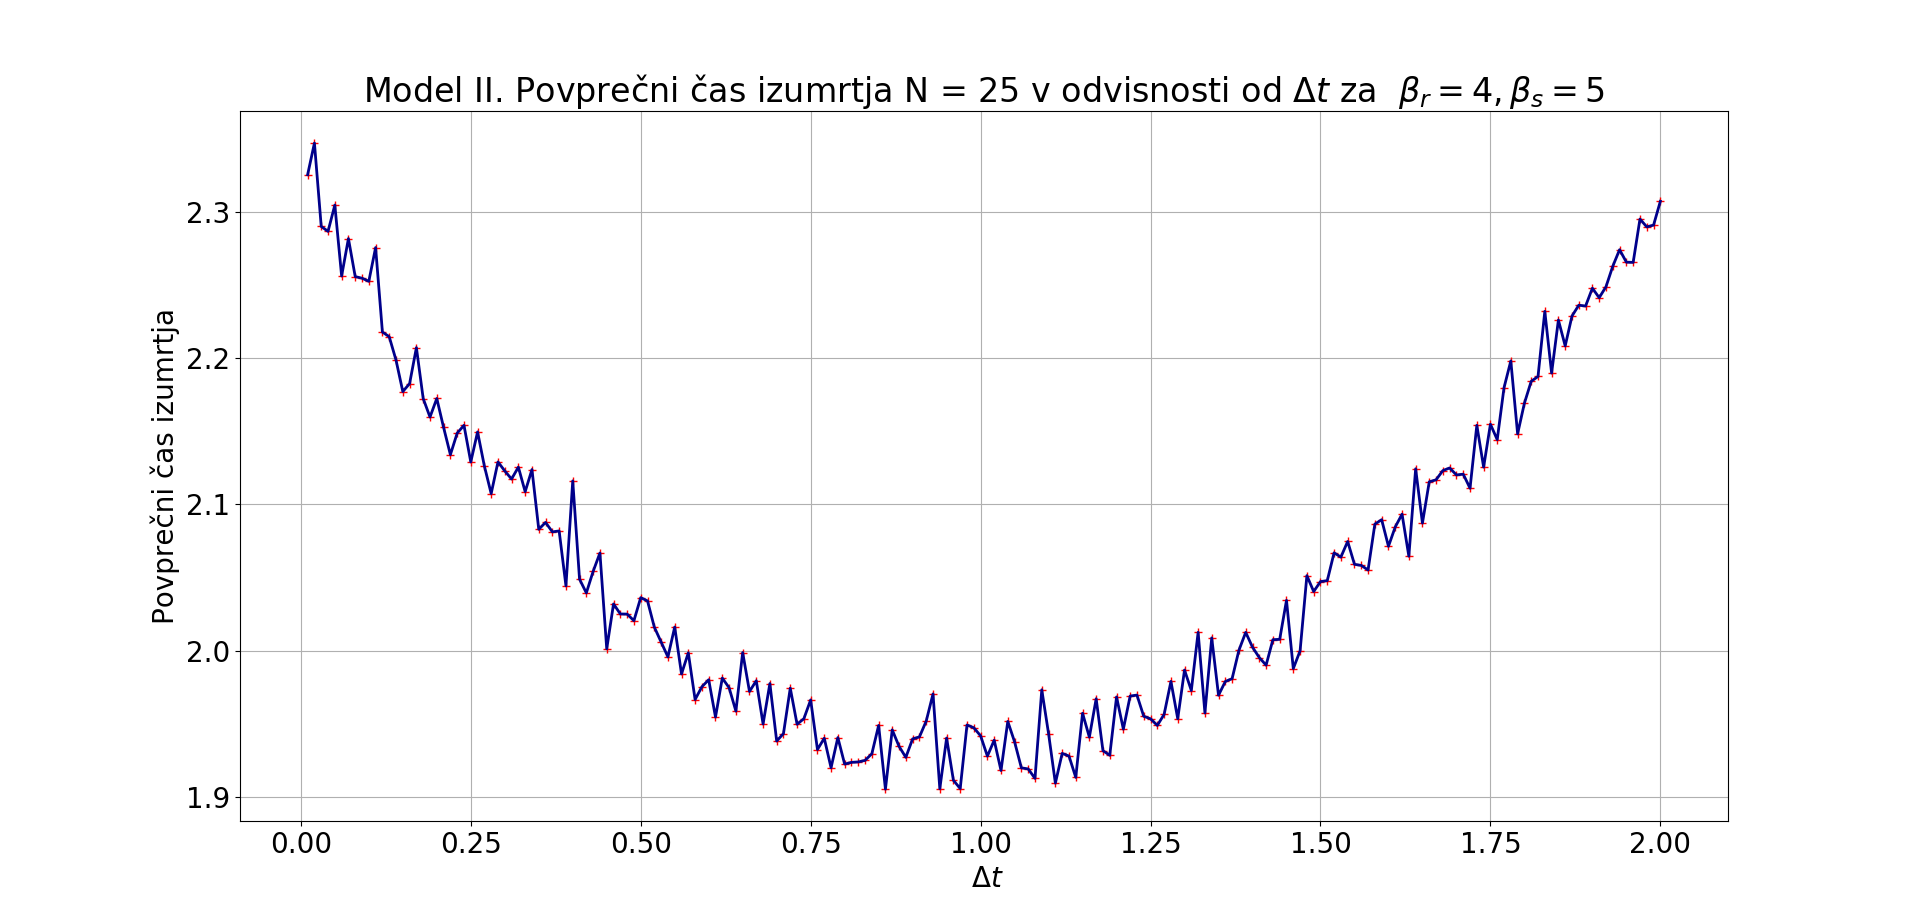
\includegraphics[width=18 cm, height=5cm]{prva_tretji_del3b.png}
     \caption{Za model II vidimo, da povprečni čas najprej pada nato pa začne rahlo naraščati z razmikom $\Delta t$, verjetno je to nefizikalno saj je razmik že prevelik za dobro simulacijo, to postano še bolj očitno pri manjši populaciji N=25, ki je še bolj občutljiva na velike razmike, saj prehitro umre.}
     \end{figure}
     \subsubsection{Odvisnost časa izumtrja od velikosti populacije}
       \begin{figure}[H]
\centering

  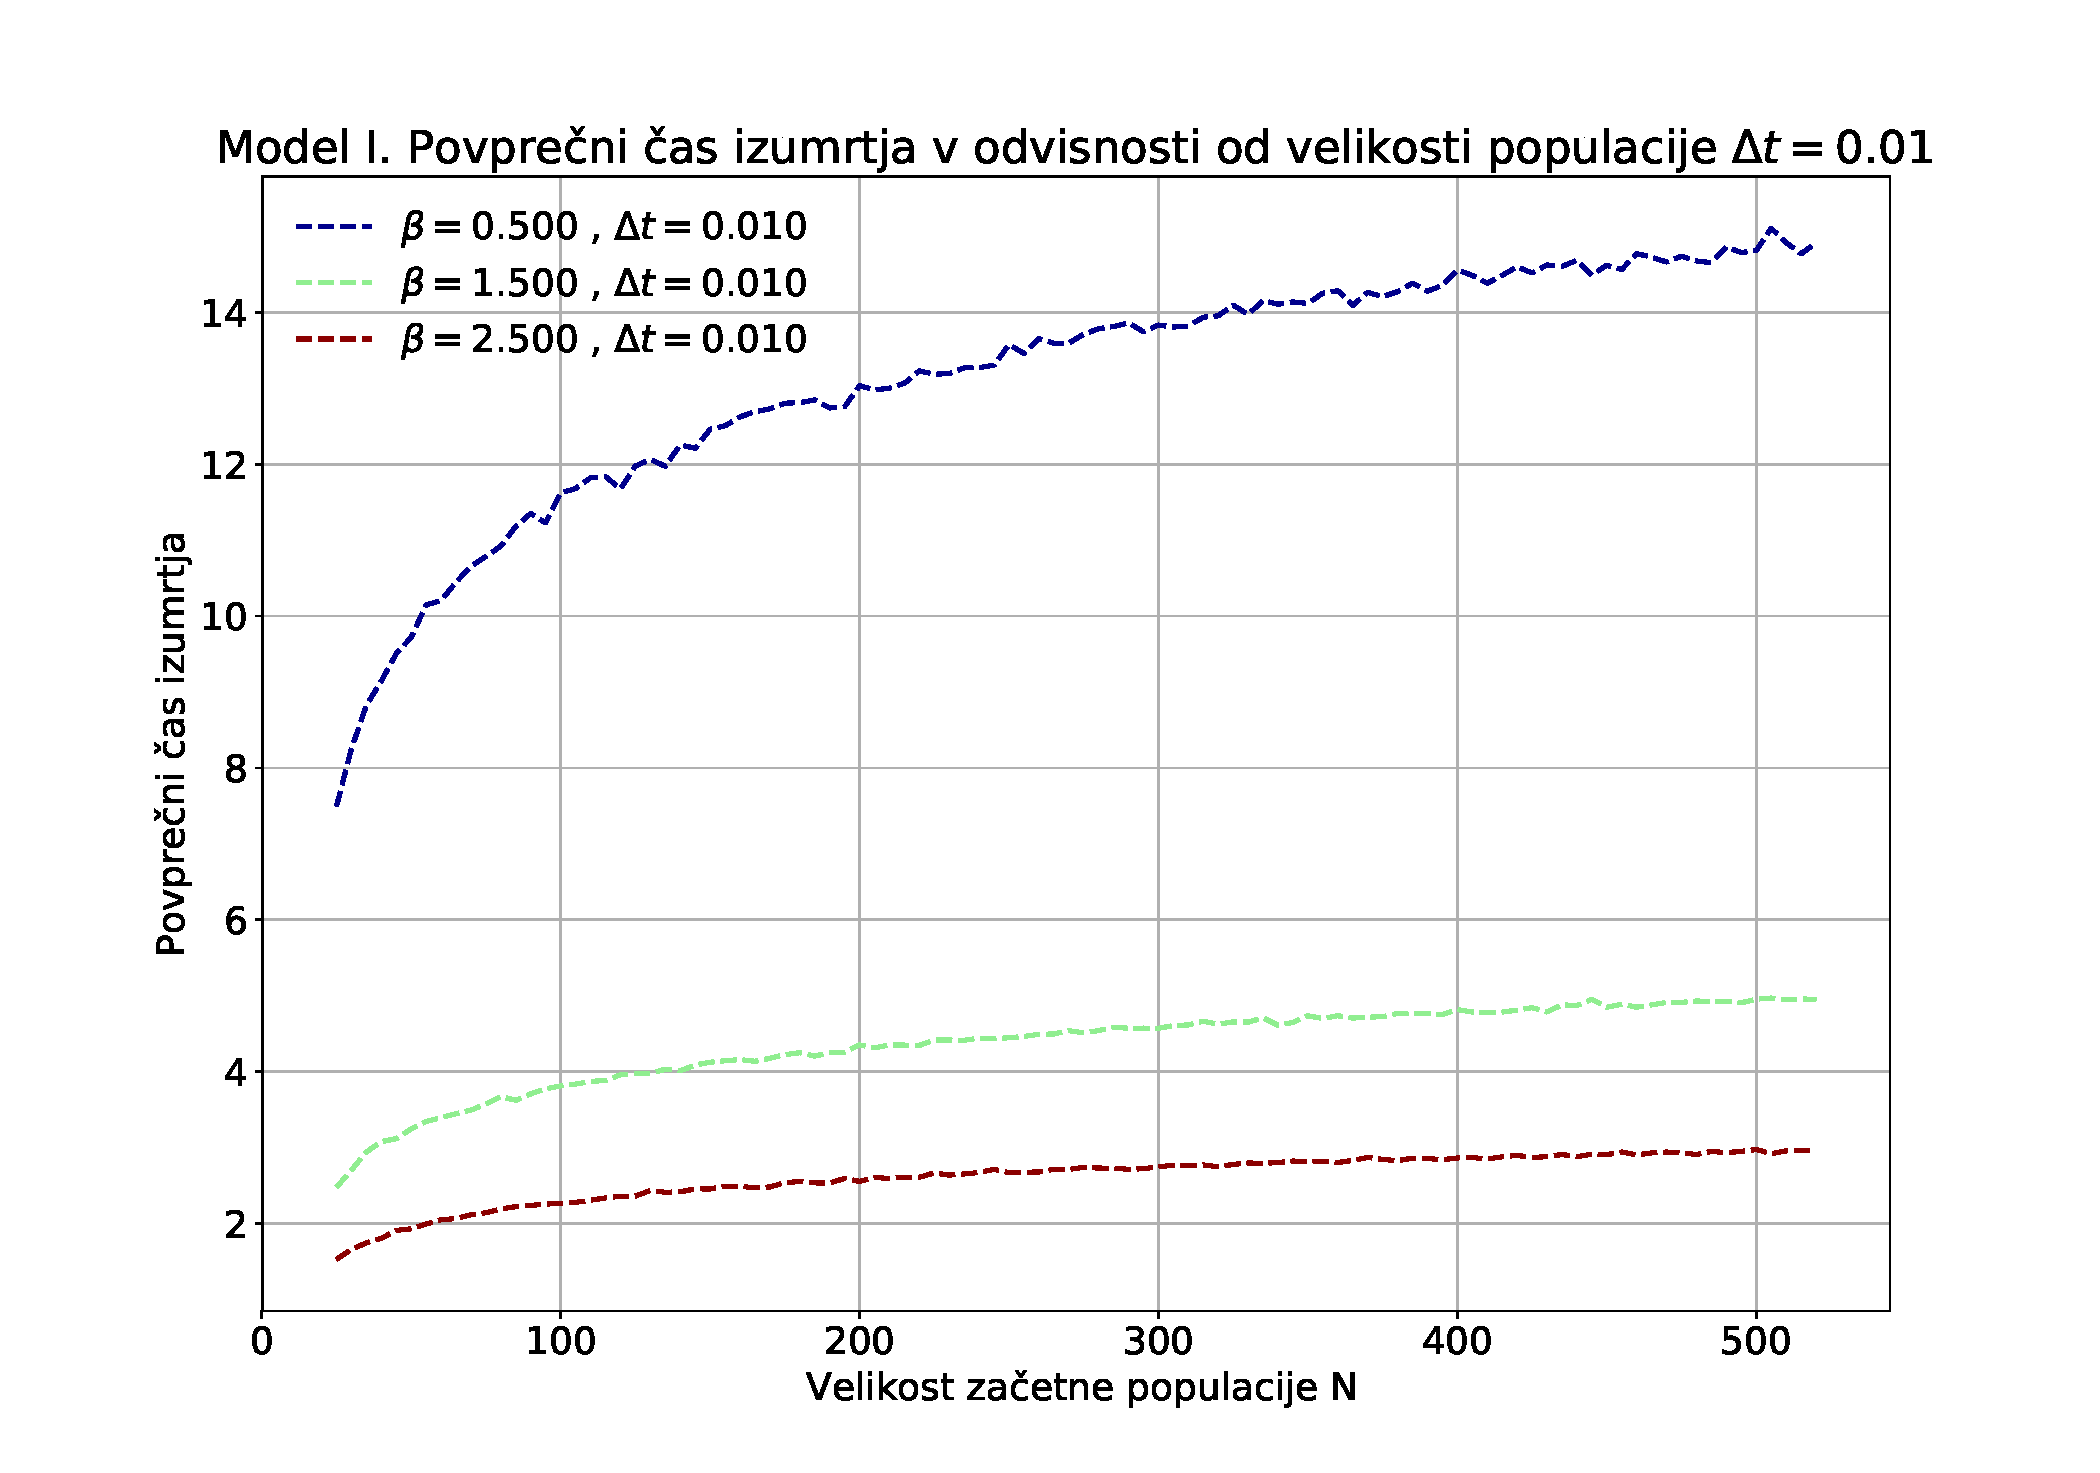
\includegraphics[width=16cm, height=8cm]{prva_velikost.pdf}

     \caption{Vidimo, da čas izumtrja na začetku strmo narašča nato pa z višjo začetno populacijo narašča vse manj strmo in konstantno. To je zaradi tega, ker ima na majhno populacijo naša konstanta smrtnosti $\beta \Delta t$ bistveno večji vpliv kot na veliko.}
     \end{figure}
 \subsection{Eksponetni model}
Če uporabimo enačbo
\begin{equation}
\frac{dN}{dt} = + \beta_r N
\end{equation}
opisujemo eksponetno naraščanje populacije, npr. bakterij.
\begin{figure}[H]
\centering

  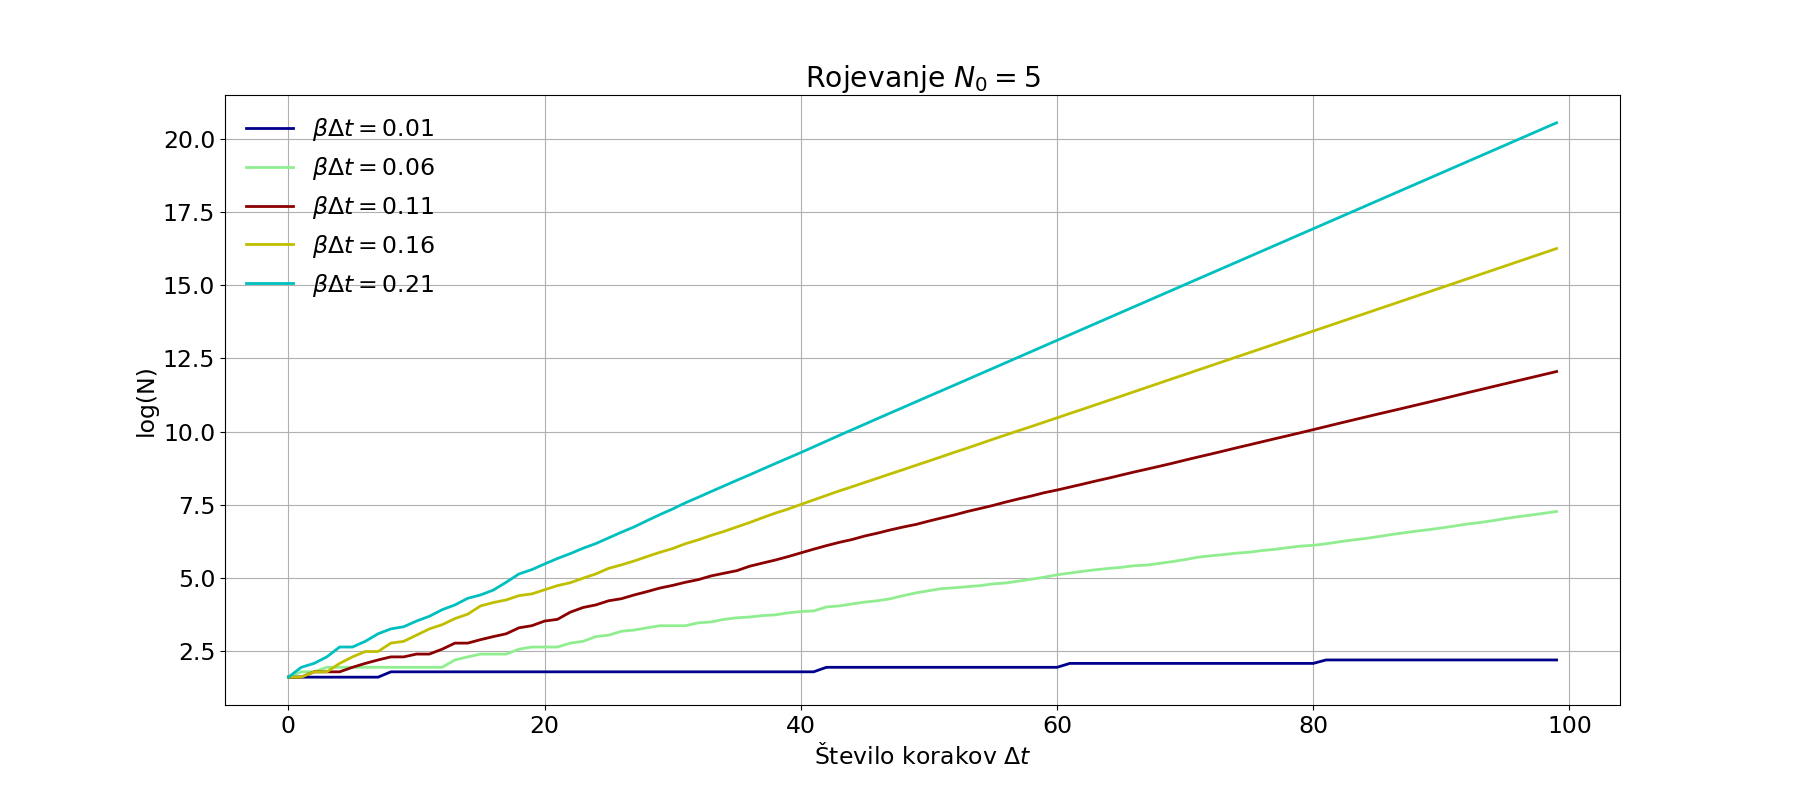
\includegraphics[width=18cm, height=4.5cm]{Rojevanja_1.png}

  \caption{Eksponetno naraščanje populacije prikazano v logaritemski skali}
 \end{figure}
 Tu ni smisla govoriti o časih izumtrja, saj populacija narašča v večnost.
\section{Matrika prehodov}
Poglejmo na problem v drugačni obliki. Zanima in sicer nas zanima, kako lahko stanje $\vec{X}(t+\Delta t)$ zapišemo s pomočjo stanja ob $\vec{X}(t)$, ki je vektor $(x_1,x_2,x_3,...,x_N$, kjer $x_i$ predstavlja število popoluacije v $i-tem$ razredu. Stanje pomnožimo s \textit{Matriko prehodov} sestavimo tako, da predpostavimo, da se lahko v enem koraku $\Delta t$ zgodi samo en dogodek - bodisi 1 osebek umre, bodisi se 1 osebek rodi, bodisi se nič ne zgodi. Tako dobimo matriko
\[
\mathcal{M} = 
\begin{bmatrix}
    1 - (R_0+S_0)\Delta t  & S_1 \Delta t  & 0 & \dots  & 0 \\
    R_0 \Delta t & 1(R_1+S_1)\Delta t & S_2 \Delta t & \dots  & 0 \\
    \vdots & \vdots & \vdots & \ddots & S_n \Delta t \\
    0 & 0 & 0 & R_{n-1}\Delta t  & 1 - (R_n + S_n)\Delta t
\end{bmatrix},
\]
ki torej predstavlja operacijo 
\begin{equation}
\vec{X}(t+\Delta t) = \mathcal{M}\vec{X}(t).
\end{equation}
Najprej si lahko ogledamo primer iz prejšnje naloge in upoštevamo parametra $S$ in $R$ enaka pri vseh $n$, torej $S= \beta_s* n$ in $R= \beta_r* n$, kjer sta $k_1$ in $k_2 $ konstante ter $n$ število razreda.
Poglejmo si potek stanja $\vec{X}(t)$.

 \begin{figure}[H]
\centering

  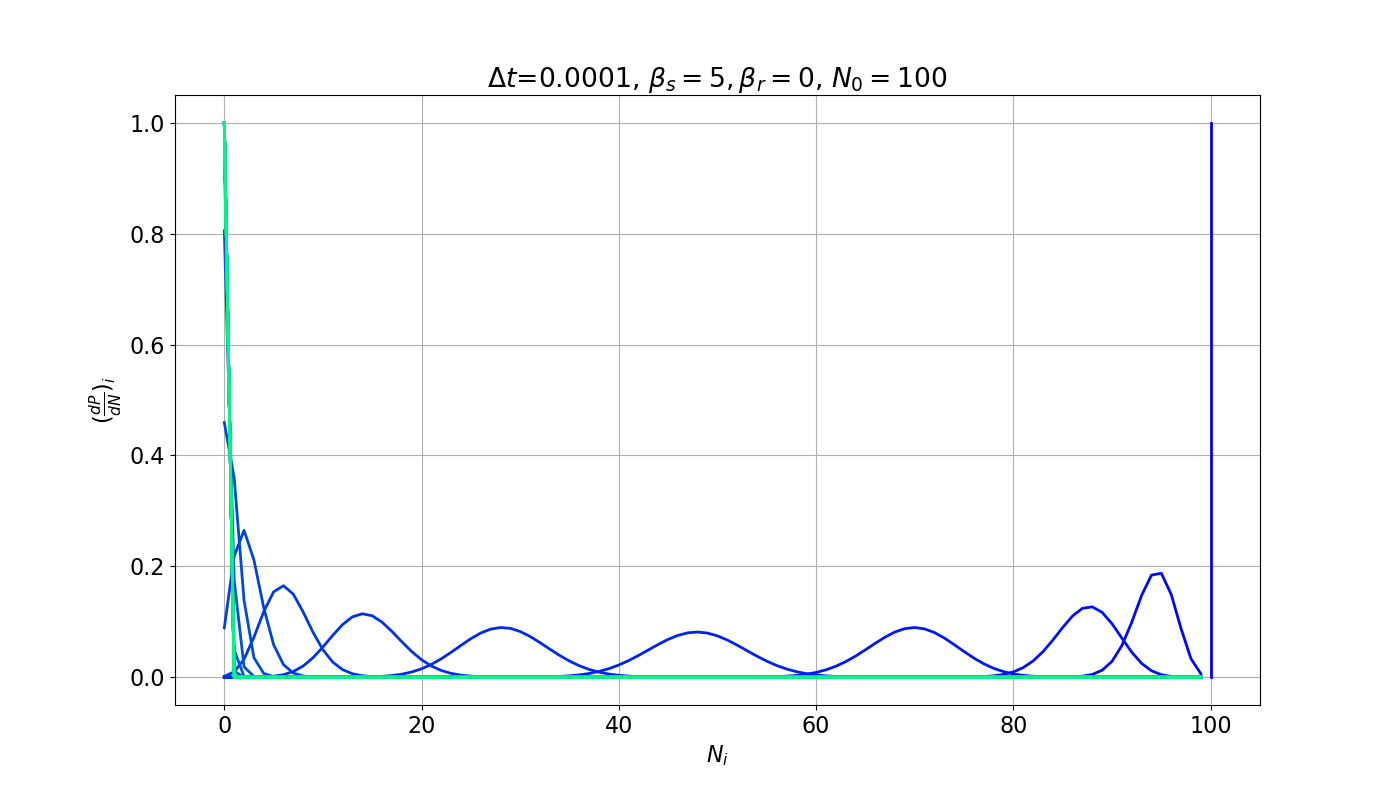
\includegraphics[width=16cm, height=6cm]{druga_1.png}
  \caption{Potek stanj sistema za N=100. Svetlejša barva pomeni kasnejši sistem. Vidimo da gre iz osnovne delta funckije pri $N_0 = 100$ stanja v drugo delta funckijo pri $N=0$, ko vsi umrejo.}

   
 \end{figure}
Iz slednjega grafa lahko beležimo dvoje \newline
\textbf{1. Povprečni razred porazdelitve ob določenem času}
\newline
\textbf{2. Povprečna ražširjenost (varianca) porazdelitve ob določenem času.}
\subsection{Povprečni razred porazdelitev}
Če je kaj pravice, bi morala diskretna shema s Poissonskim procesom in matrika prehoda podati isti rezultat, če vstavimo iste parametre.
\begin{figure}[H]
\centering

  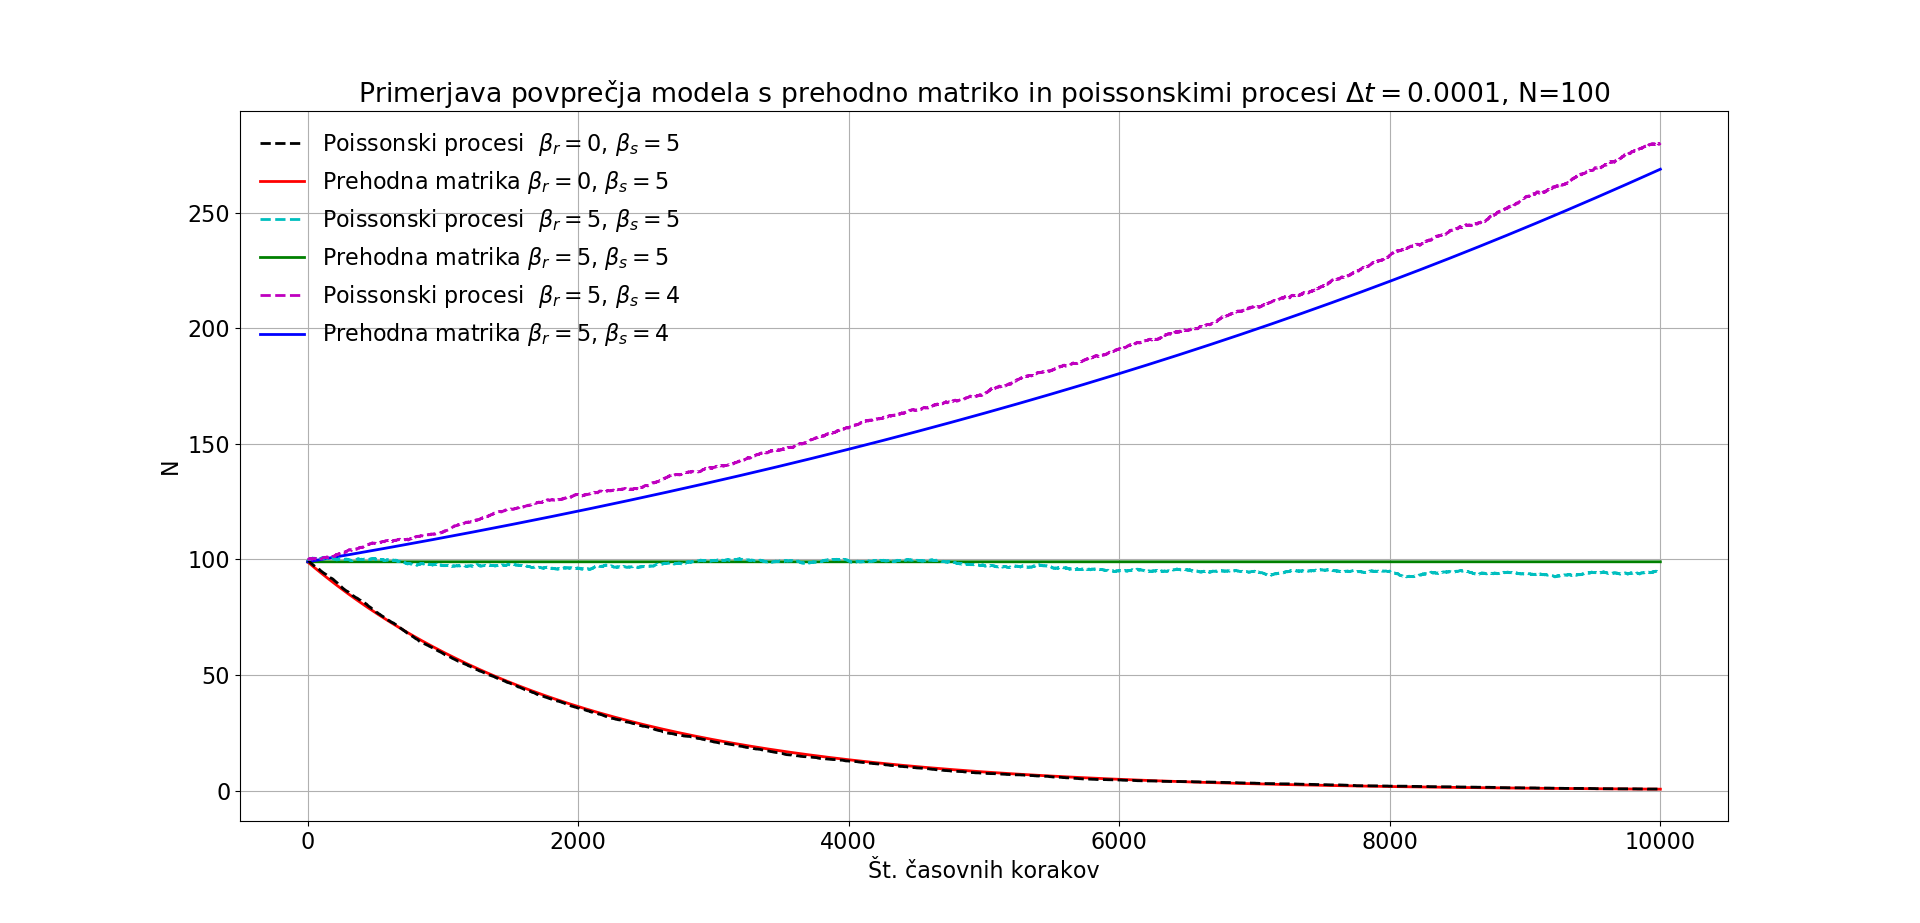
\includegraphics[width=18cm, height=10cm]{druga_2.png}
  \caption{Povprečni razredi v določenem času prehodne matrike (za n= 10 meritev), ter povprečno število populacije v določenem času (n = 40 meritev). Za $\beta_r =0 ,\beta_s=5$ je prileganje veliko boljše, saj so fluktuacije Poissonskih procesov manjše, kot za $\beta_r =5,\beta_s=4$. To je bilo opazno tudi pri prvem delu naloge. }

   
 \end{figure}
 \subsection{Varianca porazdelitev}
Oglejmo si varianco porazdelitev za populacijo $N = 100$ in $N= 250$.
 \begin{figure}[H]
\centering

  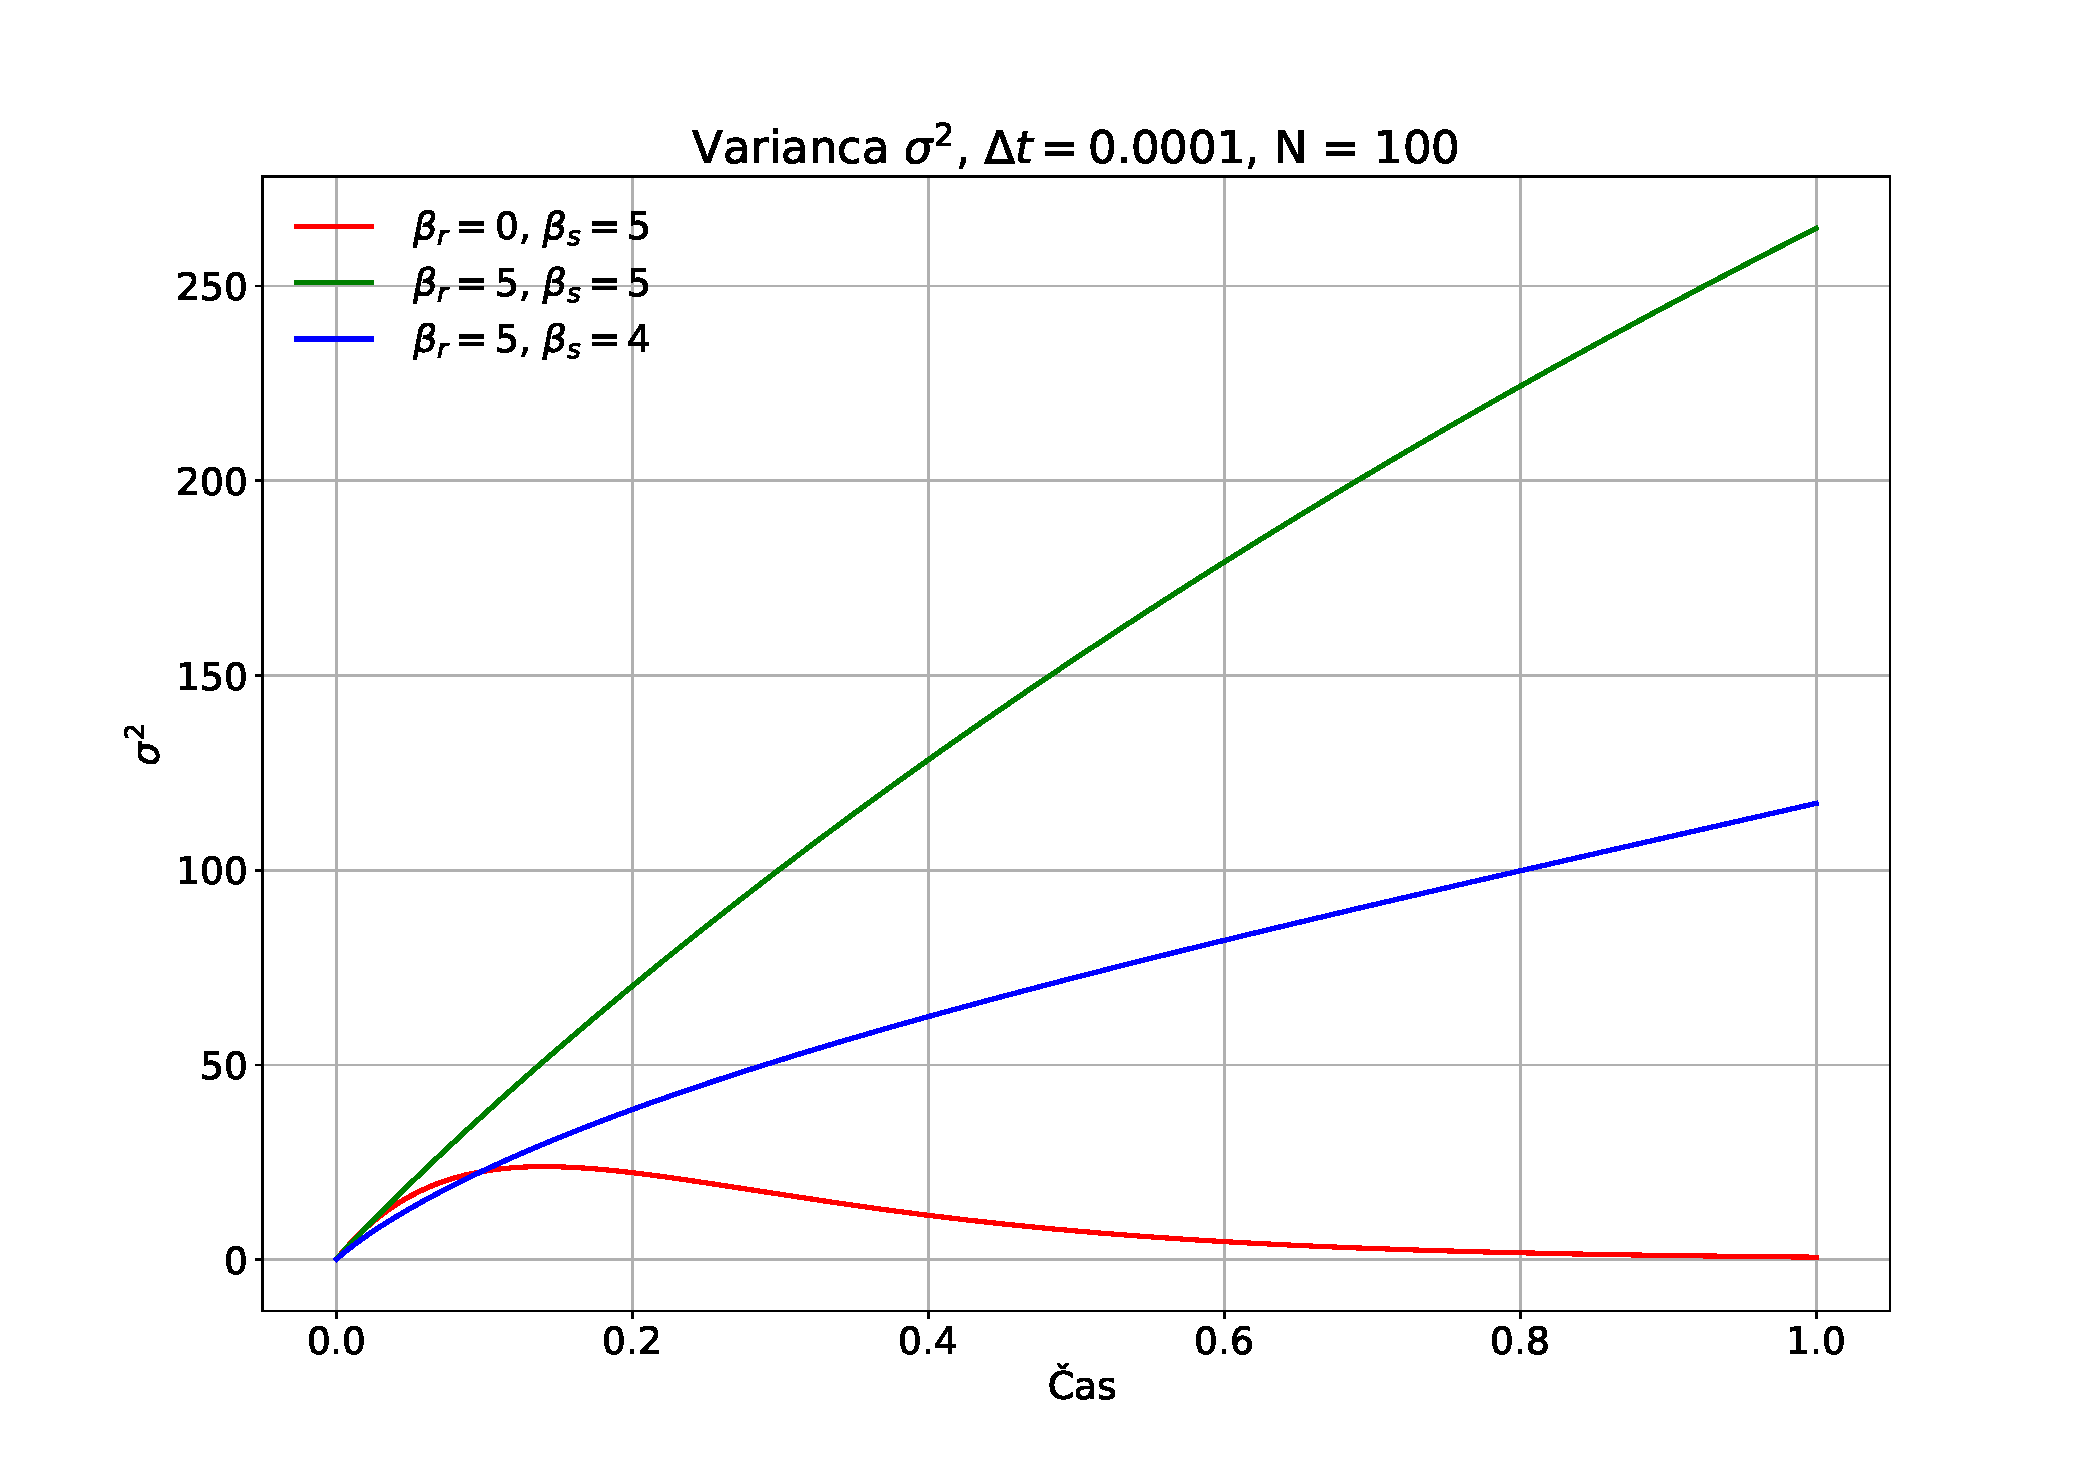
\includegraphics[width=15cm, height=5.5cm]{druga_3.pdf}
    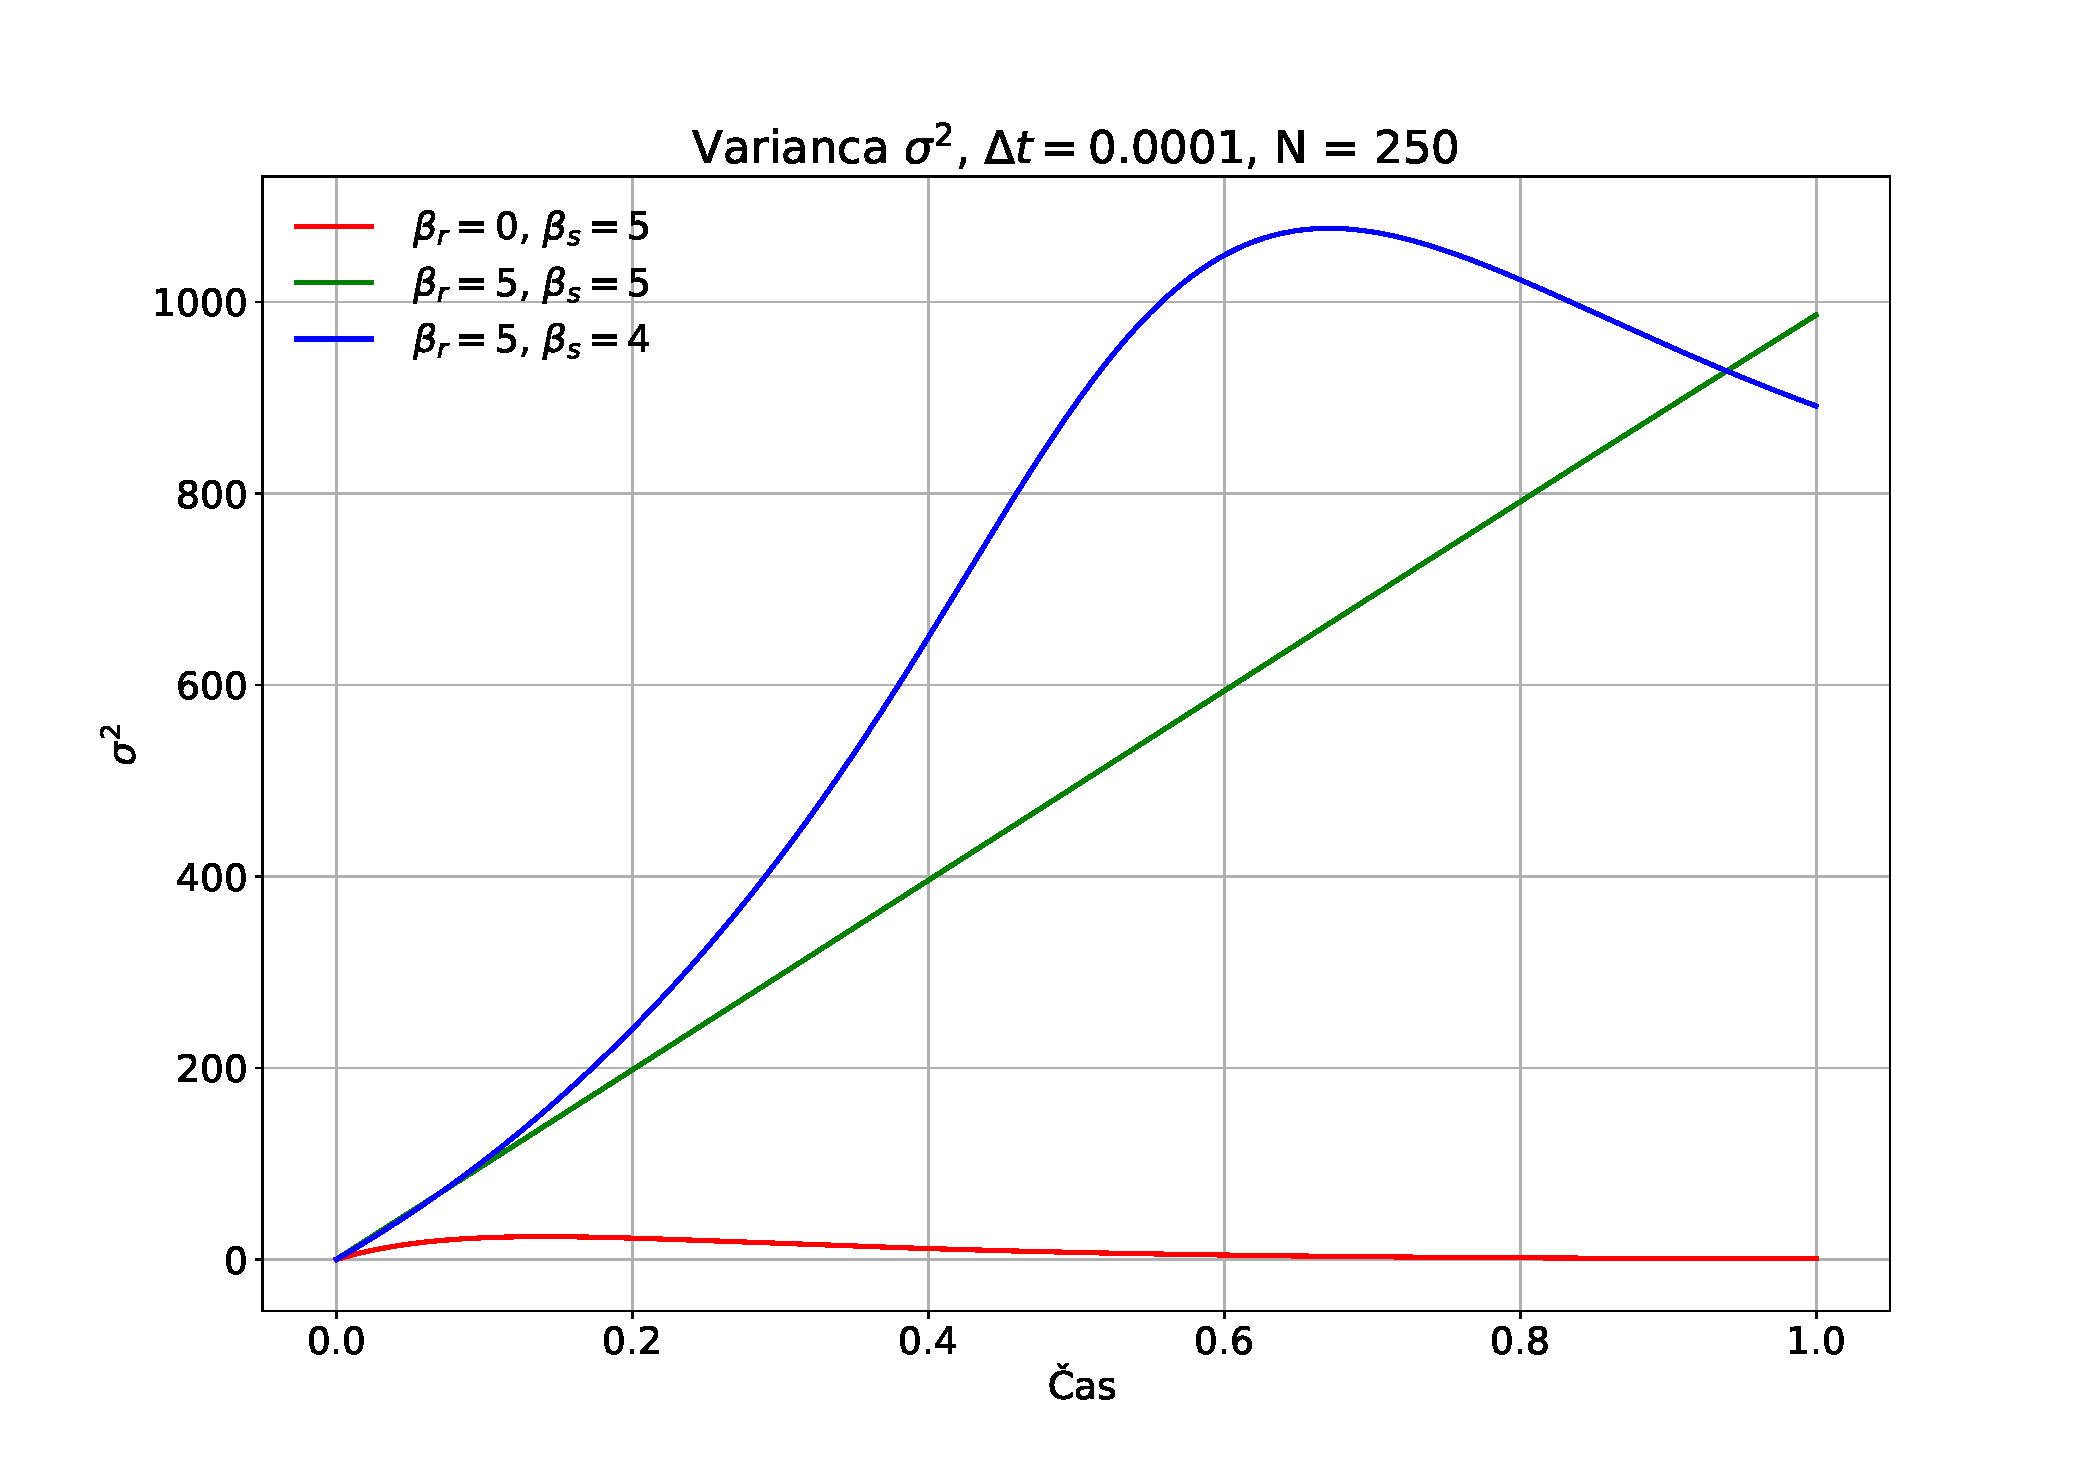
\includegraphics[width=15cm, height=5.5cm]{druga_4.pdf}

  \caption{Varianca v odvisnosti od časa različne modele in začetne populacije. Vidimo, da pri umirajočem modelu razpreščenost pada najprej narašča in nato pada, saj vsi umrejo in postane stanje 0 najbolj verjetno. Med tem, ko se pri modelu z rojstvi in smrti varianca veča in postajajo verjetnosti za stanja vse bolj razpršena.}

   
 \end{figure}
 \section{Zajci in lisice}
Obravnavamo še stohastični model zajcev in lisic in določimo povprečno življenjsko dobo sistema, če začnemo v ravnovesnem stanju. Za stacionarno stanje velja $Z_0=200$ zajci, $L_0=50$ lisice in razmerje rodnost/smrtnost $\rho_z/\rho_L=5/4$ za zajce ter obratno za lisice. Sistem enačb za populacijski model se glasi
\begin{equation}
\dot{Z} = \rho_Z Z -\sigma_Z Z - \gamma ZL,
\end{equation}
\begin{equation}
\dot{L} = \rho_L L - \sigma_L L - \delta ZL
\end{equation}
Prepišemo ga lahko v brezdimenzijsko obliko 
\begin{equation}
\dot{Z} = 5\alpha Z - 4\alpha Z - \frac{\alpha}{L_0}ZL,
\end{equation}
\begin{equation}
\dot{L} = 4\beta L - 5\beta L + \frac{\beta}{Z_0}ZL.
\end{equation}
\textit{Stohastični model} lahko z upoštevanjem zvez s predavanj za poenostavitev $\gamma=\frac{\alpha}{L_0}$ in $\delta = \frac{\beta}{L_0}$ zapišemo kot
\begin{equation}
Z_{n+1} = Z_{n} + P(5\alpha Z_n \Delta t) - P(4\alpha Z_n \Delta t) - P(\frac{\alpha}{L_0} Z_n L_n \Delta t),
\end{equation}
kjer seveda velja $Z_{n+1}=Z(t+\Delta t)$ in $Z_n=Z(t)$ ter za lisice
\begin{equation}
L_{n+1} = L_{n} + P(4\beta L_n \Delta t) - P(5\beta L_n \Delta t) + P (\frac{\beta}{Z_0} Z_n L_n \Delta t),
\end{equation}
kjer je $L_{n+1}=L(t+\Delta t)$ in $L_n=L(t)$, P pa Poissonova porazdelitev. Vzamemo vrednosti $\alpha =1$ in $\beta = 2 $, torej se plen bolj množi kot plenilci.
\subsection{Simulacija s tremi Poissonskimi žrebi}
Simulacija traja dokler ne izumre ena od vrst (zajci ali lisice). Poglejmo si kakšne so rešitve
\begin{figure}[H]
\centering

  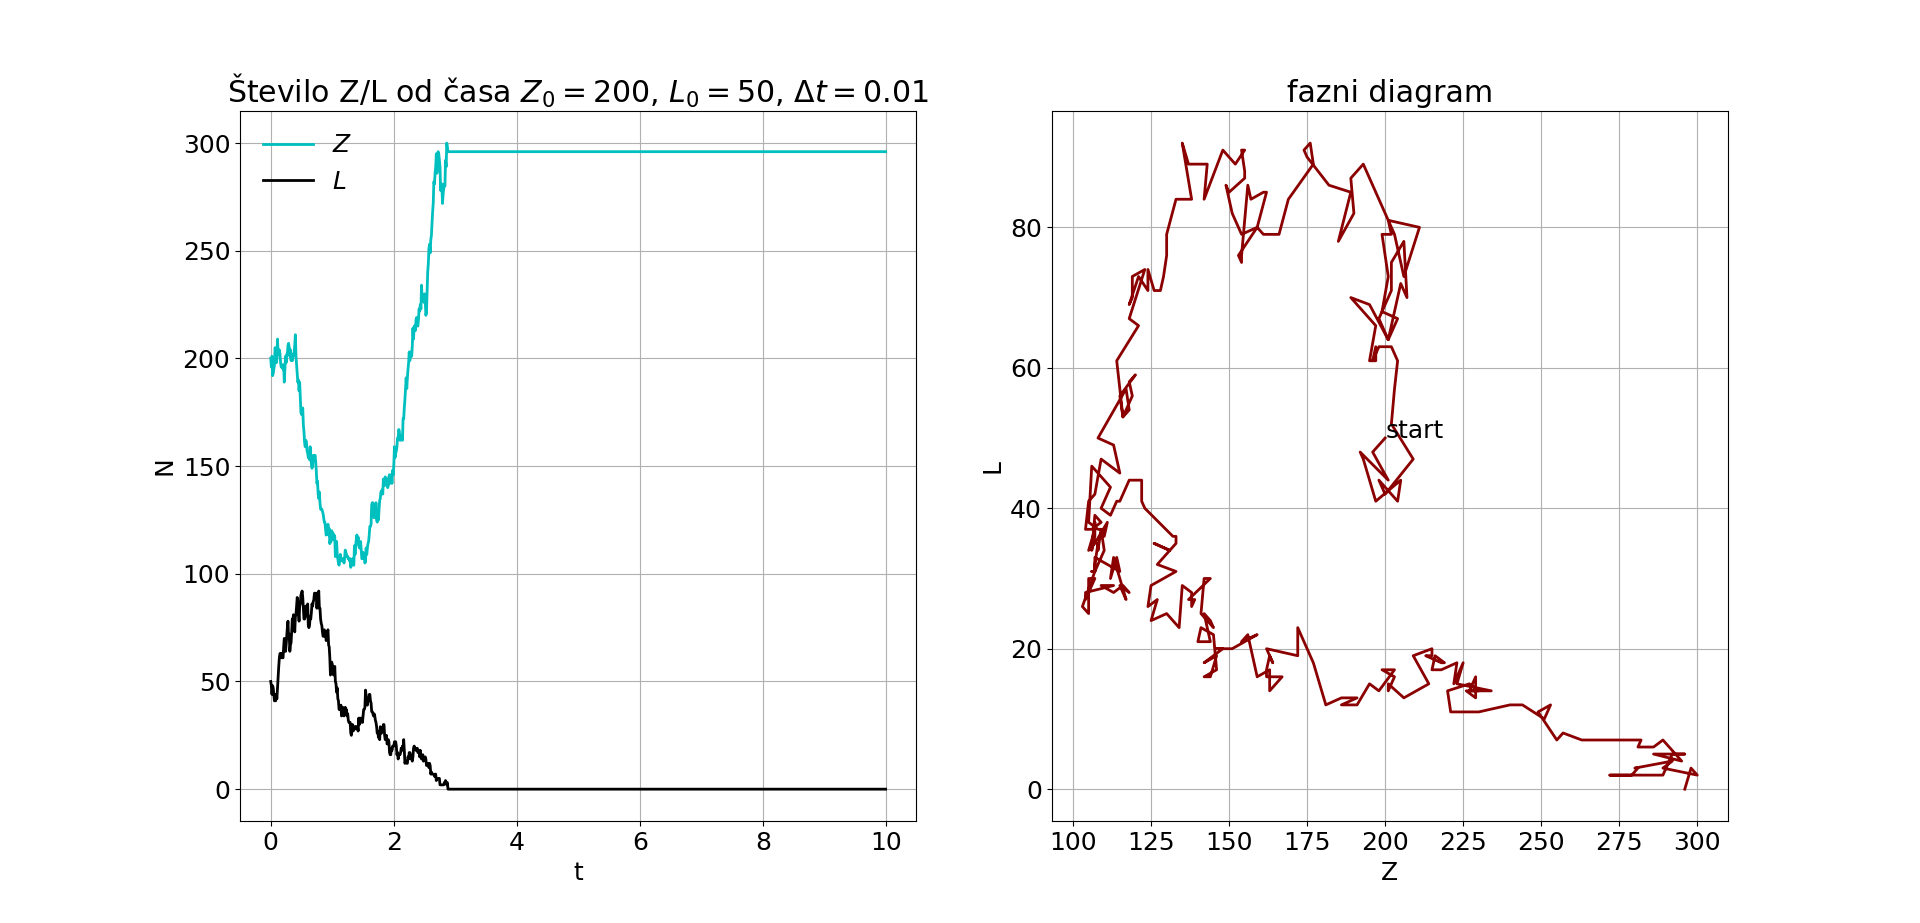
\includegraphics[width=18cm, height=6cm]{tretja_1.png}
  \caption{Poissonski proces za $Z_0 = 200 , L_0 = 50$. Na začetku smo res v stacionarni točki, nato pa nas fluktuacije odnesejo stran iz nje.}

   
 \end{figure}
 Rešitve močno fluktuirajo, že npr. ponovni zagon simulacije nam da čisto nov sprehod po faznem prostoru.
 \begin{figure}[H]
\centering

  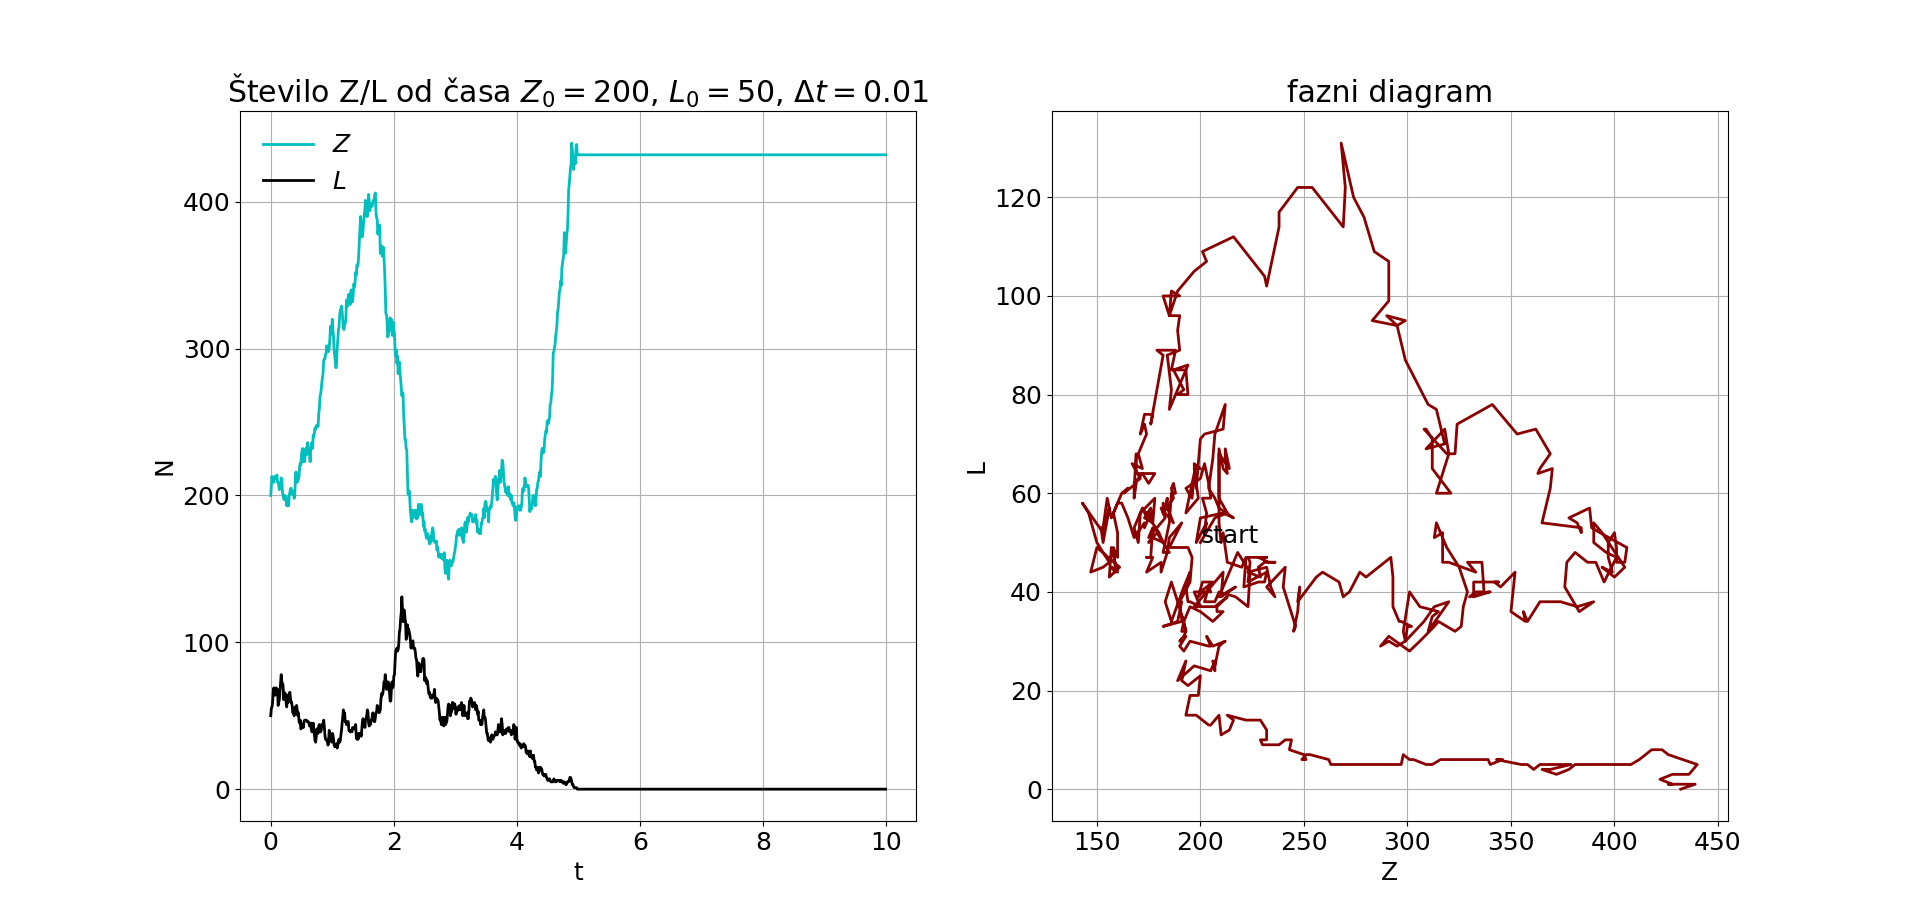
\includegraphics[width=18cm, height=6cm]{tretja_2.png}
  \caption{Poissonski proces za $Z_0 =200, L_0 = 50$.}

   
 \end{figure}
 Poglejmo še kaj se zgodi ko vstavimo $Z_0=L_0=100$, pričakujemo daljše obhodne dobe.
 \begin{figure}
   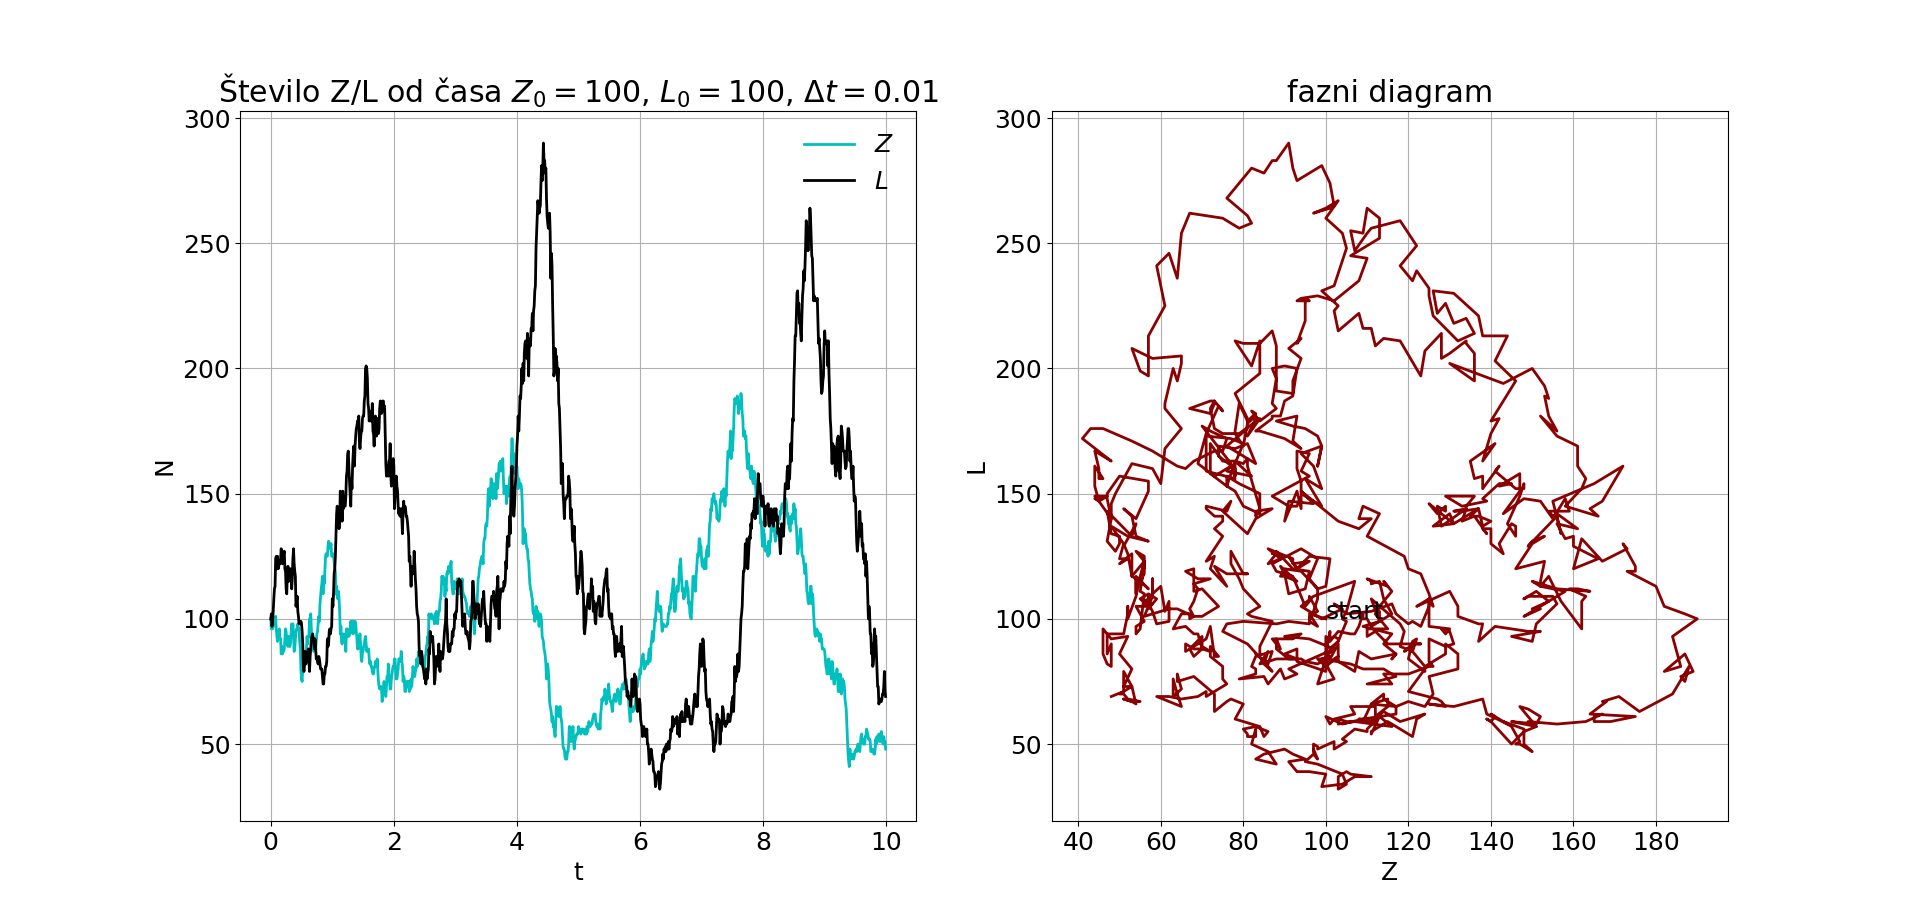
\includegraphics[width=18cm, height=6cm]{tretja_3.png}
  \caption{Poissonski proces za $Z_0 = 100 , L_0 = 100$.}

   
 \end{figure}
 Rešitve močno fluktuirajo, že npr. ponovni zagon simulacije nam da čisto nov sprehod.
 \begin{figure}[H]
\centering

  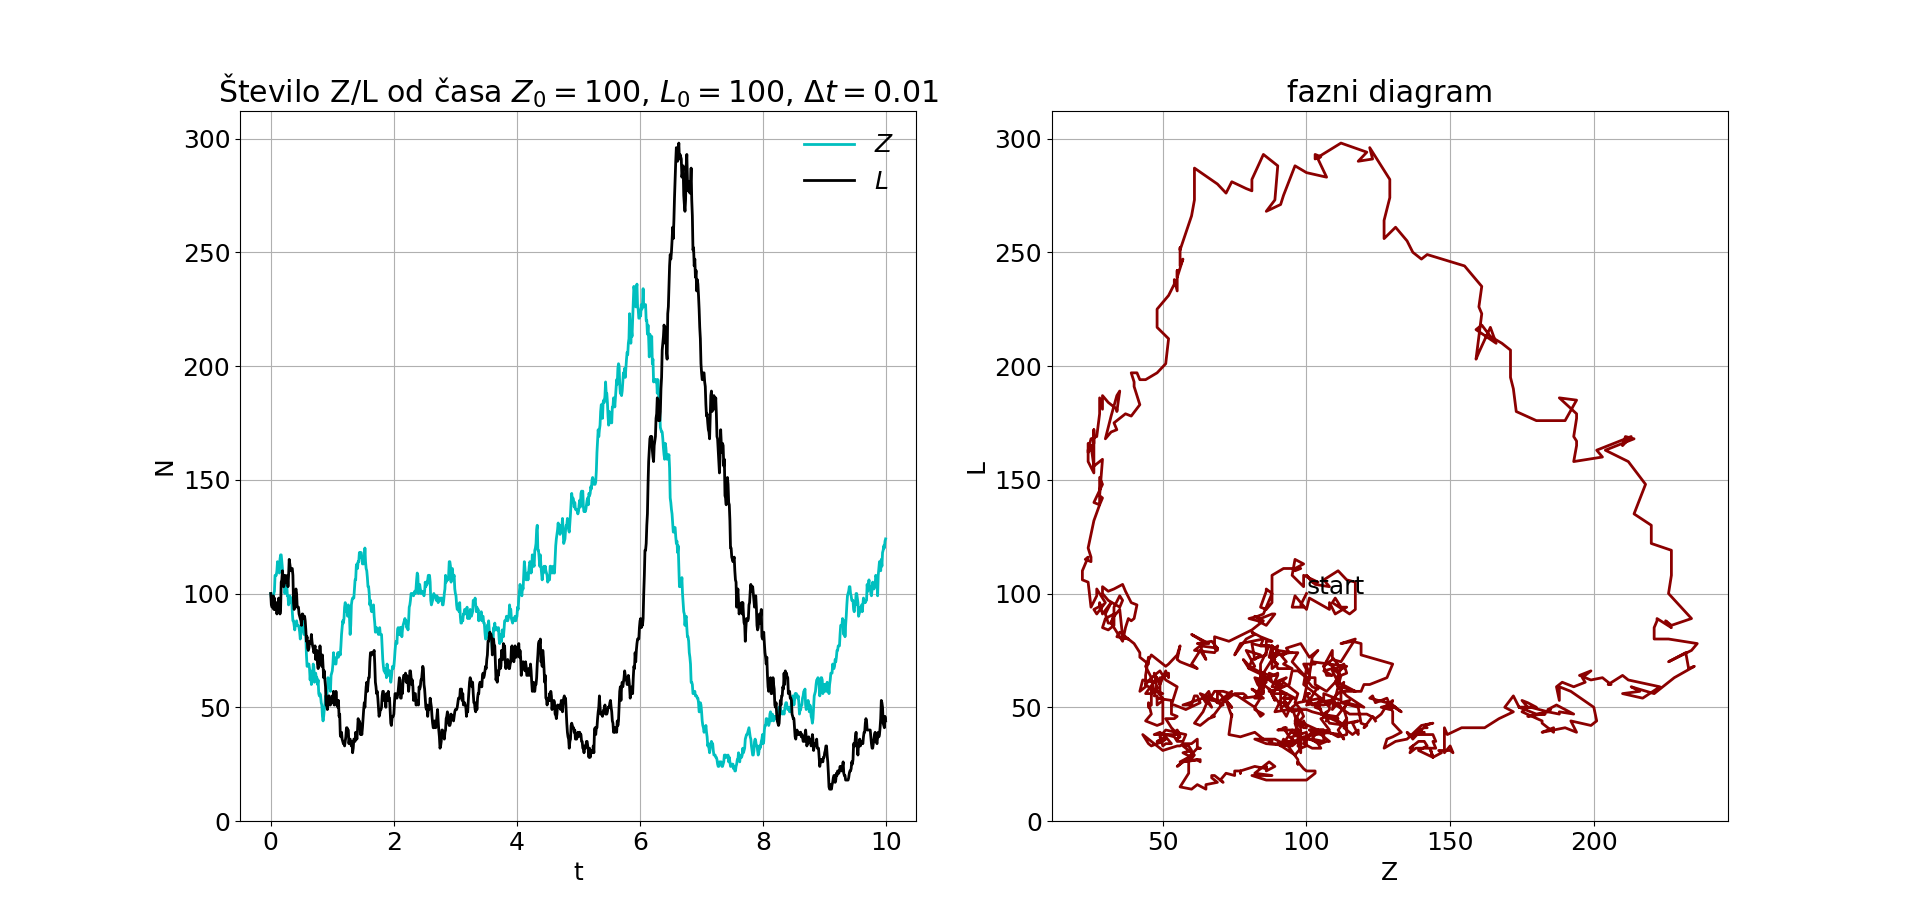
\includegraphics[width=18cm, height=6cm]{tretja_4.png}
  \caption{Poissonski proces za $Z_0 =100, L_0 = 100$.}  

   
 \end{figure}
 Vidimo, da je preživetje res daljše, in da je tudi umiranje bolj naključno. Seveda takšno rešitev lahko dobimo tudi iz stacionarne točke, le bolj redka je.
\subsection{Povprečna življenska doba sistema}
Simulirajmo proces 1000-krat in si shranjujmo čas življenjske dobe sistema ter ga prikažimo na histogramu.
 \begin{figure}[H]
\centering

  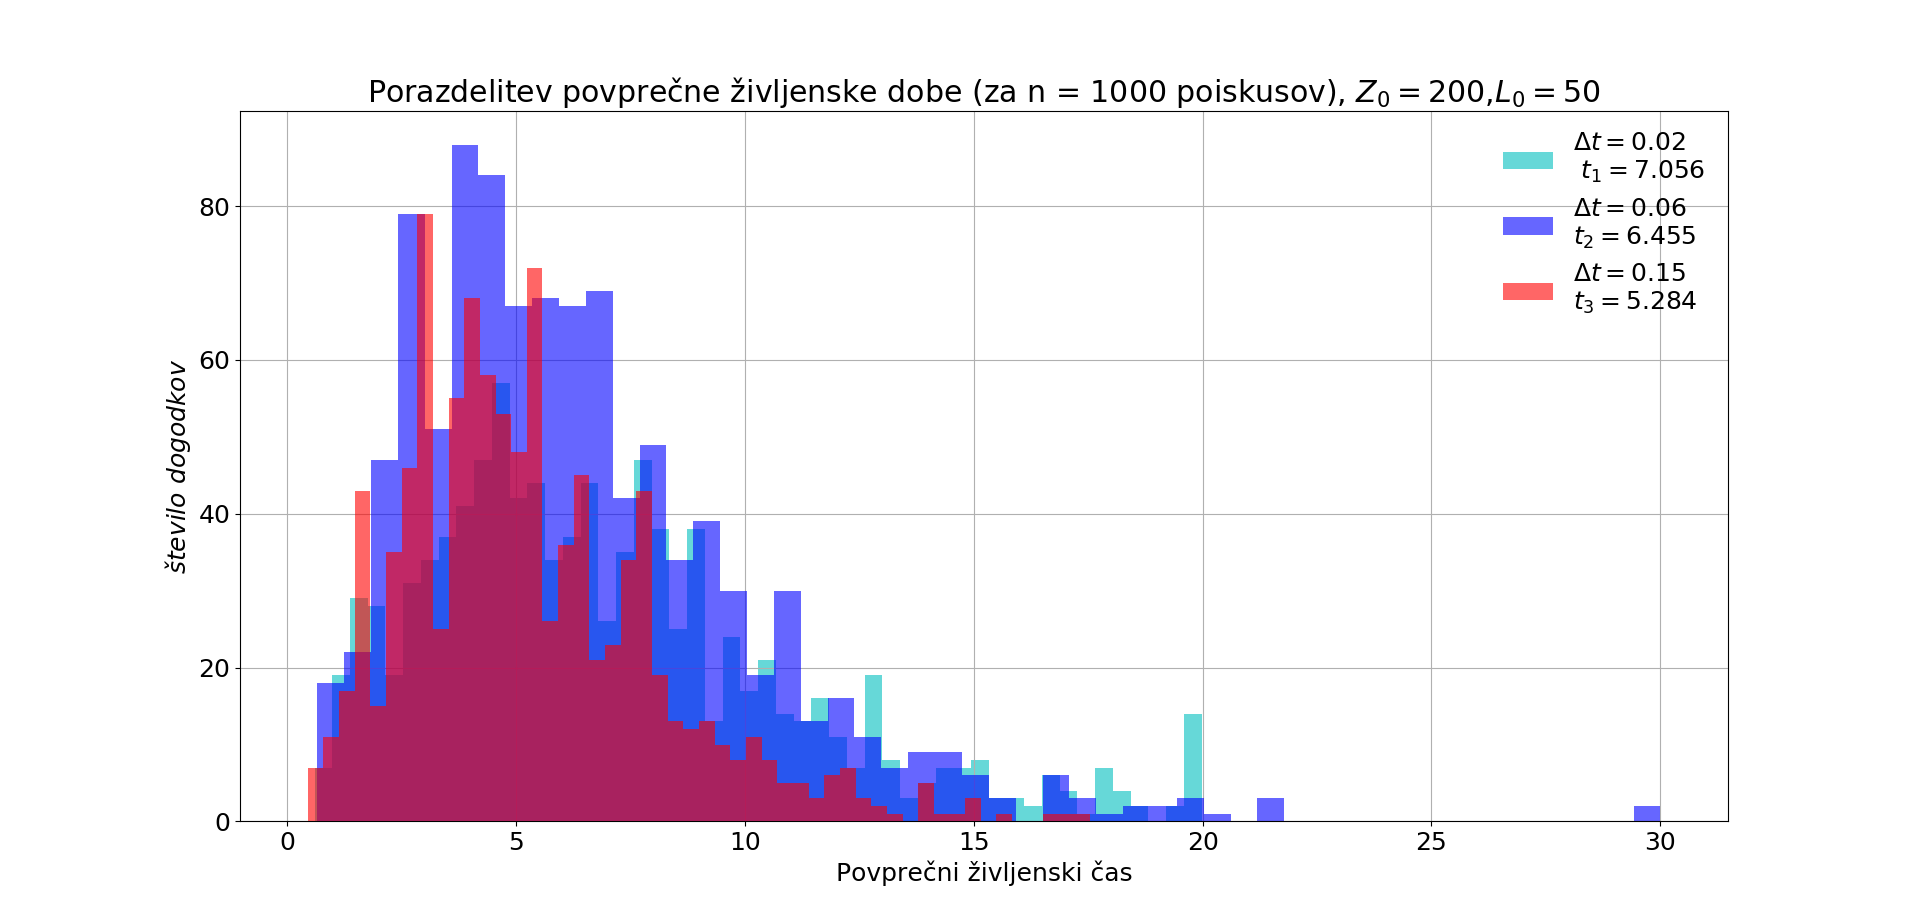
\includegraphics[width=16cm, height=6cm]{tretja_6.png}
  \caption{Izačunana povprečna življenska doba sistema za dva koraka $\Delta t = 0.02 $ in $\Delta t = 0.1$. Vidimo da korak vpliva na sistem tako, da je povprečna življenska doba krajša, a ne močno. torej lahko določimo povprečen življenjski čas sistema, kot povprečje vseh treh} 
   
 \end{figure}
 \textbf{ Povprečni čas sistema Zajci-lisice pri stacionarni točki ($Z_0 = 200, L_0 = 50$) znaša $t = 6.265  \pm 0.725$} 
 \subsection{Sklopljeni sistem}
Kaj pa če sistema iz enačbe (13) in (14) sklopimo, tako da združimo Poissonski proces 
\begin{equation}
Z_{n+1} = Z_{n} + P(\alpha Z_n \Delta t) -P(\frac{\alpha}{L_0} Z_n L_n \Delta t),
\end{equation}

\begin{equation}
L_{n+1} = L_{n} + P(-\beta L_n \Delta t) + P (\frac{\beta}{Z_0} Z_n L_n \Delta t),
\end{equation}
Pričakujemo, da bo zaradi le enega žreba fluktuacij manj in se zato sistem tudi dlje časa ne bo ustavil.
 \begin{figure}[H]
\centering

  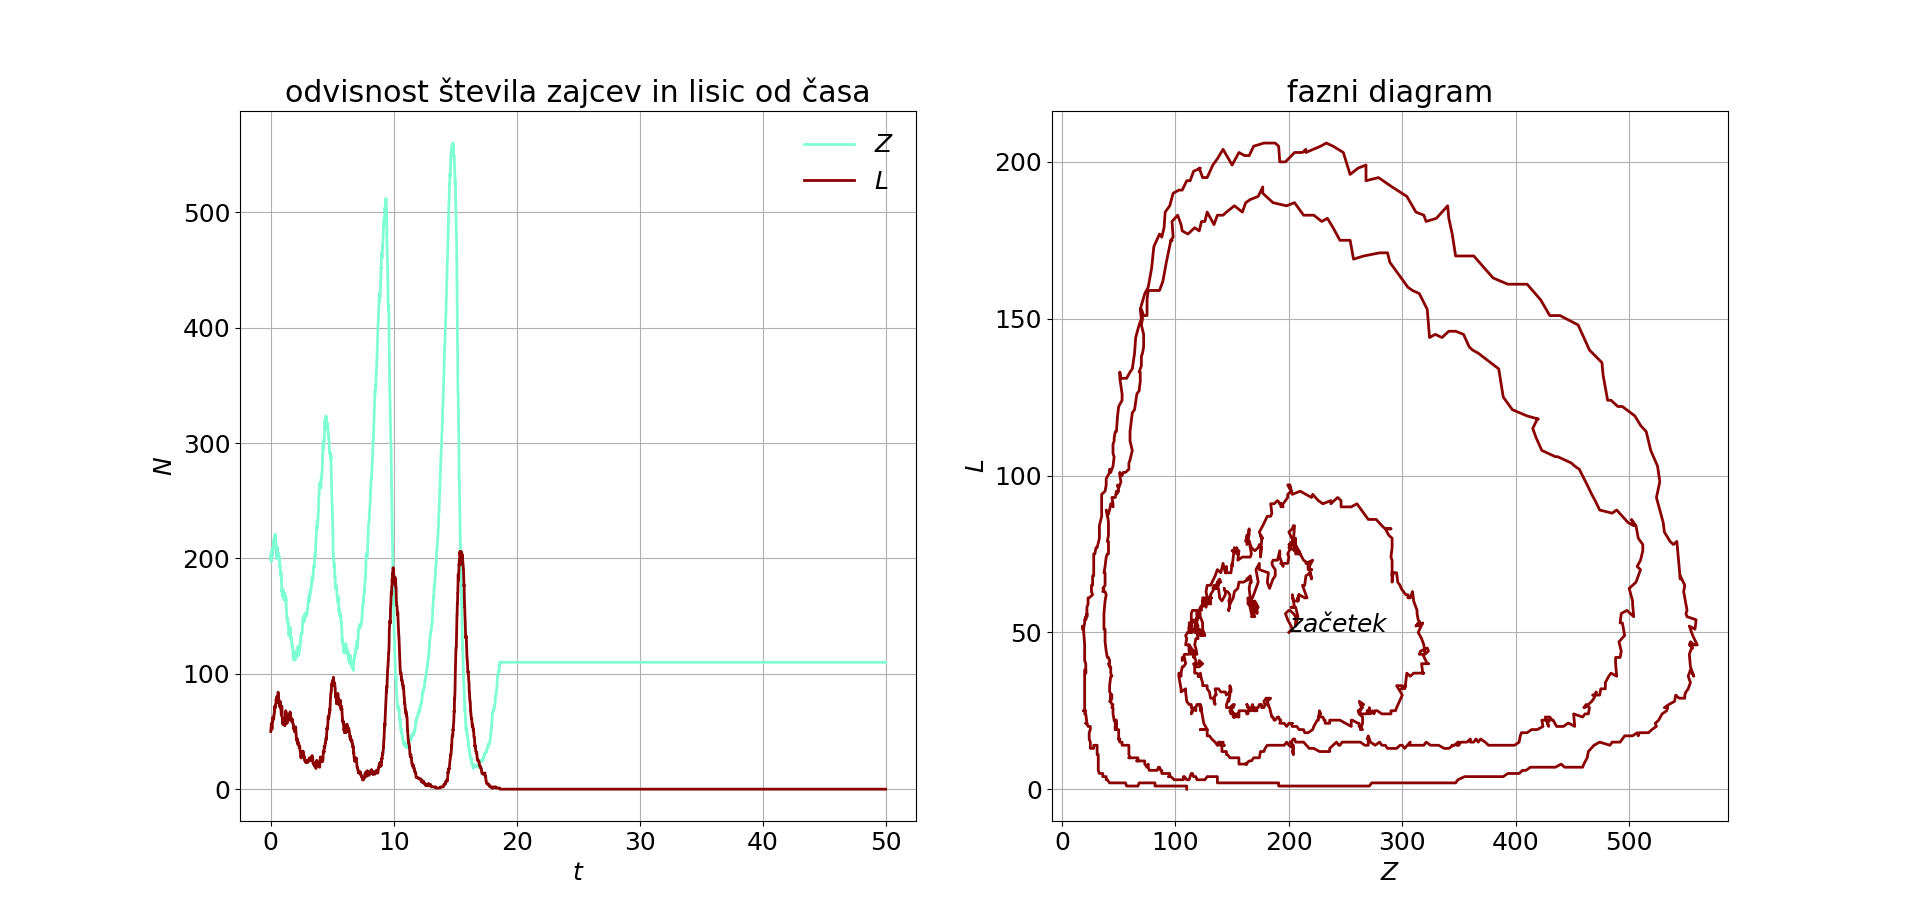
\includegraphics[width=16cm, height=6cm]{tretja_8.png}

   
 \end{figure}
 \begin{figure}[H]
\centering

  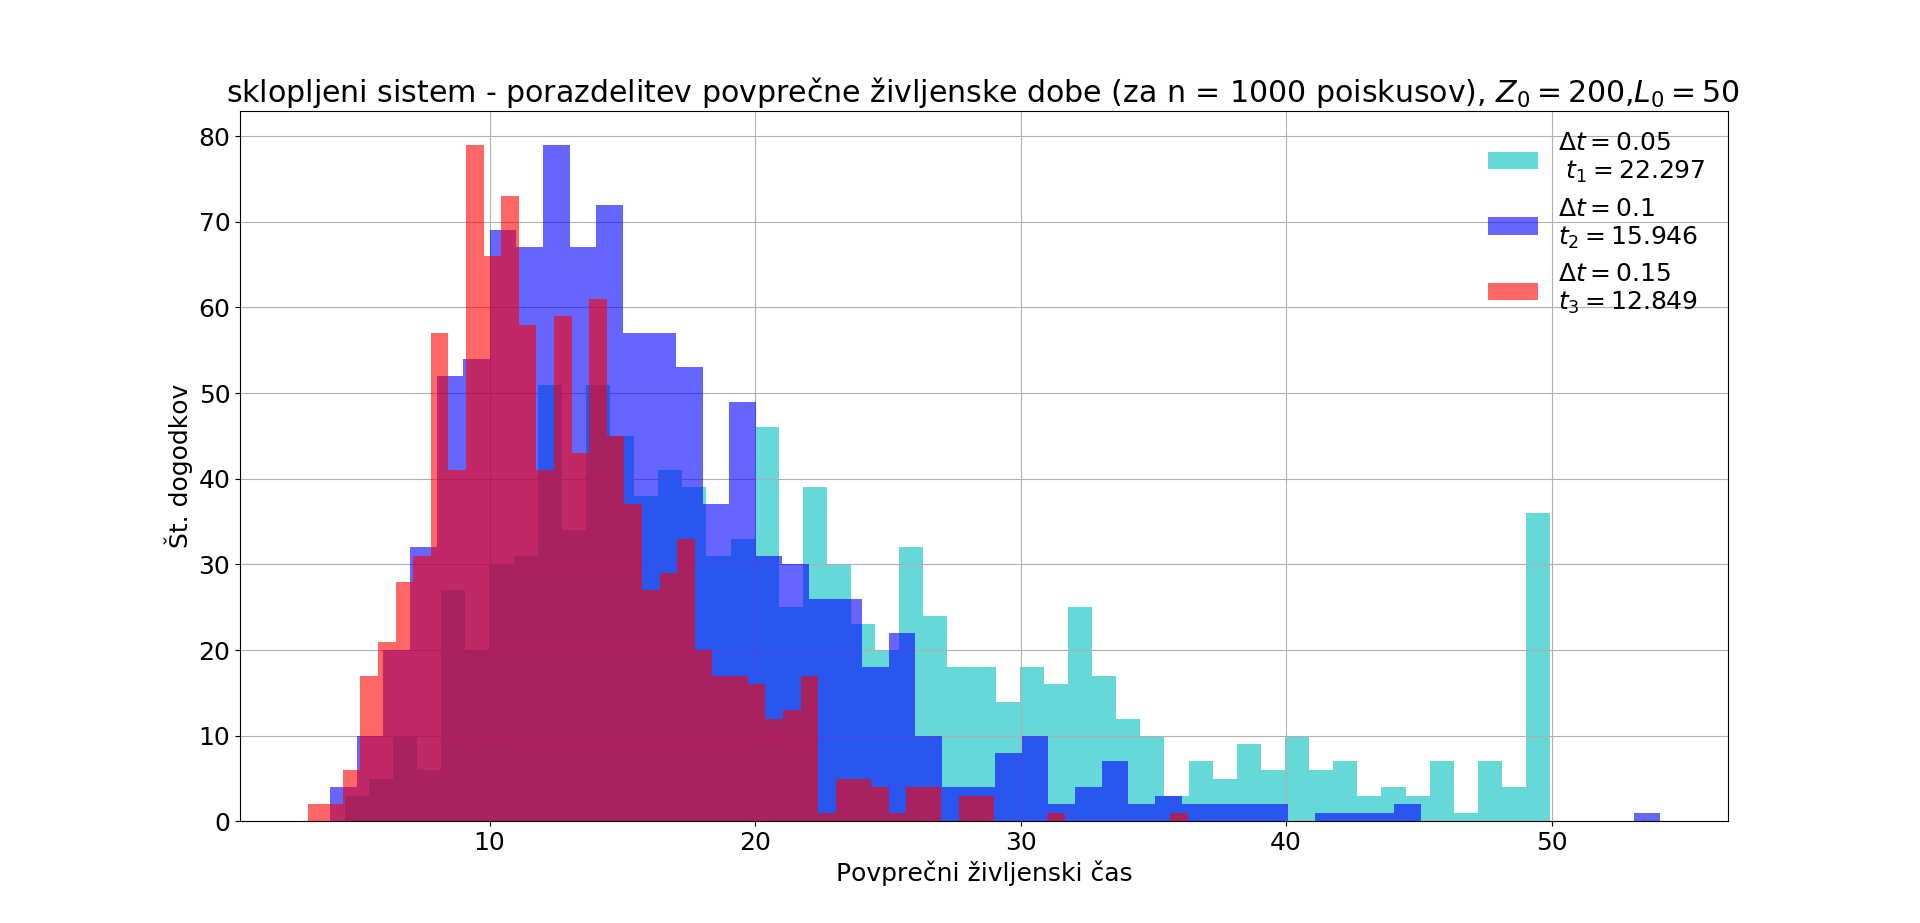
\includegraphics[width=16cm, height=6cm]{tretja_7.png}
  \caption{Tu se povprečni življenjski časi precej razlikujejo, zato jih ne moremo izpovprečiti, hkrati pa so fluktuacije manjše in zato povprečni časi daljši. Verjetno se zdi, da je bolj pravilen proces ne skopljenega sistema, saj upošteva rojstvo in smrt kot neodivsen dogodek, med tem ko jih pri sklopljenem sistemu izpovprečimo v neto rojstvo /smrt.}  


   
 \end{figure}

\fi


\section{Zaključek}
Naučili smo se stohastičen opis populacijskih modelov in opis populacijskih modelov s pomočjo matrike prehodov. Zanimivo se mi je zdelo, da lahko s poissonskimi procesi simuliramo tudi fluktuacije v naravi.


\end{document}